% ============================================================
%  Lab 1: Brushless Motor Characterization and Control
%  Actuators and Robotic Design, Fall 2026
%
%  Structure follows the handout exactly: every P and Q question
%  appears as its own numbered block, in the order written there.
%  Fill in the marked slots; delete the guidance comments as you go.
% ============================================================

\documentclass[11pt]{article}

% ---------- page ----------
\usepackage[margin=1in]{geometry}
\usepackage{parskip}
\setlength{\parskip}{0.6em}

% ---------- maths ----------
\usepackage{amsmath, amssymb}
\usepackage{siunitx}
\sisetup{
  per-mode            = symbol,
  range-units         = single,
  detect-weight       = true,
  group-separator     = {,},
  group-digits        = integer   % never group the decimal part
}
% handy shorthands used throughout
\DeclareSIUnit\rev{rev}
\DeclareSIUnit\count{count}
\DeclareSIUnit\lsb{LSB}

% ---------- figures and tables ----------
\usepackage{graphicx}
\usepackage{array}      % provides \extrarowheight
\usepackage{booktabs}
\usepackage{float}
\usepackage[font=small, labelfont=bf]{caption}
\usepackage{subcaption}

% ---------- code listings (for the odd config line) ----------
\usepackage{listings}
\usepackage{xcolor}
\lstset{
  basicstyle   = \ttfamily\small,
  breaklines   = true,
  frame        = single,
  rulecolor    = \color{gray!40},
  backgroundcolor = \color{gray!5},
  columns      = fullflexible,
  keepspaces   = true
}

% ---------- links ----------
\usepackage[colorlinks=true, linkcolor=blue!50!black,
            citecolor=blue!50!black, urlcolor=blue!50!black]{hyperref}

% ============================================================
%  Question environment
%  Usage:  \question{Q1.1}{From the calibration output, record ...}
%  Prints a bold tag, the question text in italic, then your answer.
% ============================================================
\usepackage{mdframed}
\newcommand{\question}[2]{%
  \bigskip
  \noindent\textbf{#1}\quad{#2}\par\nobreak\smallskip
}
% Opcode decode cell: binary groups with their field labels underneath.
% \opcell{raw}{bits1}{bits2}{bits3}{label1}{label2}{label3}
% Labels may contain \\ for line breaks.
% NOTE: \newline, not \\, for the line break -- inside a p{} column a bare
% \\ ends the table ROW and throws the inner tabular out of the cell.
\newcommand{\opcell}[7]{%
  \texttt{0x#1} in binary $\rightarrow$\par\vspace{0.35em}\noindent
  \setlength{\tabcolsep}{4pt}%
  \begin{tabular}[t]{@{}ccc@{}}
    \underline{\texttt{#2}} & \underline{\texttt{#3}} & \underline{\texttt{#4}} \\[0.2em]
    \scriptsize\shortstack{#5} &
    \scriptsize\shortstack{#6} &
    \scriptsize\shortstack{#7}
  \end{tabular}%
}
% Solution label, matching the style used in other coursework.
\definecolor{cit}{rgb}{0.05,0.2,0.45}
\newcommand{\solution}{\medskip\noindent{\color{blue}\textbf{Solution:}}\par\nobreak}

% Shorthand for a prediction block, so P answers are visually
% distinct and obviously written before the data.
\newmdenv[
  linecolor   = gray!50,
  backgroundcolor = gray!5,
  linewidth   = 0.5pt,
  skipabove   = 0.6em,
  skipbelow   = 0.6em,
  innertopmargin = 0.5em,
  innerbottommargin = 0.5em
]{prediction}

% ============================================================

\title{\textbf{Lab 1: Brushless Motor Characterization and Control}\\
       \large Actuators and Robotic Design, Fall 2026}
\date{}
\begin{document}

\maketitle
\vspace{-5em}
\begin{table}[H]
\centering
\begin{tabular}{ll}
\toprule
\multicolumn{2}{c}{\textbf{Group 5}} \\
\midrule
 Juan Cerquera Cano         &  member 1 nuid\\    
 Charles Piper              &  member 2 nuid\\
 Tapan Shashikant Patil     &  002310627\\
 Mohammed Abdullah          &  002068653\\
\bottomrule
\end{tabular}
\end{table}
% ------------------------------------------------------------



% ============================================================
\section{Bring-up and Calibration}
% ============================================================

\subsection*{Configuration and calibration output}
% Brief note on what you ran. Put the full console capture in Appendix A.

\question{P1.1}{Calibration cannot run with the shaft locked. Name at least two
quantities the tool measures that need the rotor to turn. Why does each quantity
need movement to calibrate?}

\begin{prediction}
% ANSWER
Prediction for P1.1
\end{prediction}

\question{Q1.1}{From the calibration output, record the resistance, every
inductance the tool reports, the saliency ratio, $K_v$, and the pole count.
Give both the pole count and the number of pole pairs. Which of the two does
the commutation math use?}

\solution

\begin{table}[H]
\centering
\caption{Values reported by \texttt{moteus\_tool --calibrate}.}
\begin{tabular}{llll}
\toprule
Quantity & Symbol & Value & Unit \\
\midrule
Winding Resistance      & $R$        & 0.0641 & \si{\ohm} \\
Inductance            & $L$        & \num{2.7498e-5} & \si{\henry} \\
Inductance, $d$-axis  & $L_d$      & \num{2.8487e-05} & \si{\henry} \\
Inductance, $q$-axis  & $L_q$      & \num{4.6571e-05} & \si{\henry} \\
Saliency ratio        & $L_q/L_d$  &  & --- \\
Velocity constant     & $K_v$      & 310.76  & \si{rpm\per\volt} \\
Pole count            & ---        & 14 & --- \\
Pole pairs            & $p$        &  & --- \\
\bottomrule
\end{tabular}
\end{table}

% ANSWER: which one the commutation maths uses, and why.

\question{Q1.2}{Compute the electrical time constant $L/R$ and the matching
first-order corner frequency in Hz, for the inductance labelled
\texttt{inductance} and for \texttt{inductance\_q}. Which of the two creates
torque?}

\solution

\begin{equation*}
  \tau_e = \frac{L}{R}, \qquad
  f_c = \frac{1}{2\pi\tau_e} = \frac{R}{2\pi L}
\end{equation*}

\begin{table}[H]
\centering
\caption{Electrical time constants and corner frequencies.}
\begin{tabular}{llll}
\toprule
Inductance used & $L$ & $\tau_e$ & $f_c$ \\
\midrule
\texttt{inductance} &  &  &  \\
\texttt{inductance\_q} &  &  &  \\
\bottomrule
\end{tabular}
\end{table}

\question{Q1.3}{Plot position against time. Report the peak-to-peak spread and
the standard deviation, in encoder counts and in degrees. What are some ways
that encoder noise could propagate through a control loop?}

\solution

\begin{figure}[H]
  \centering
  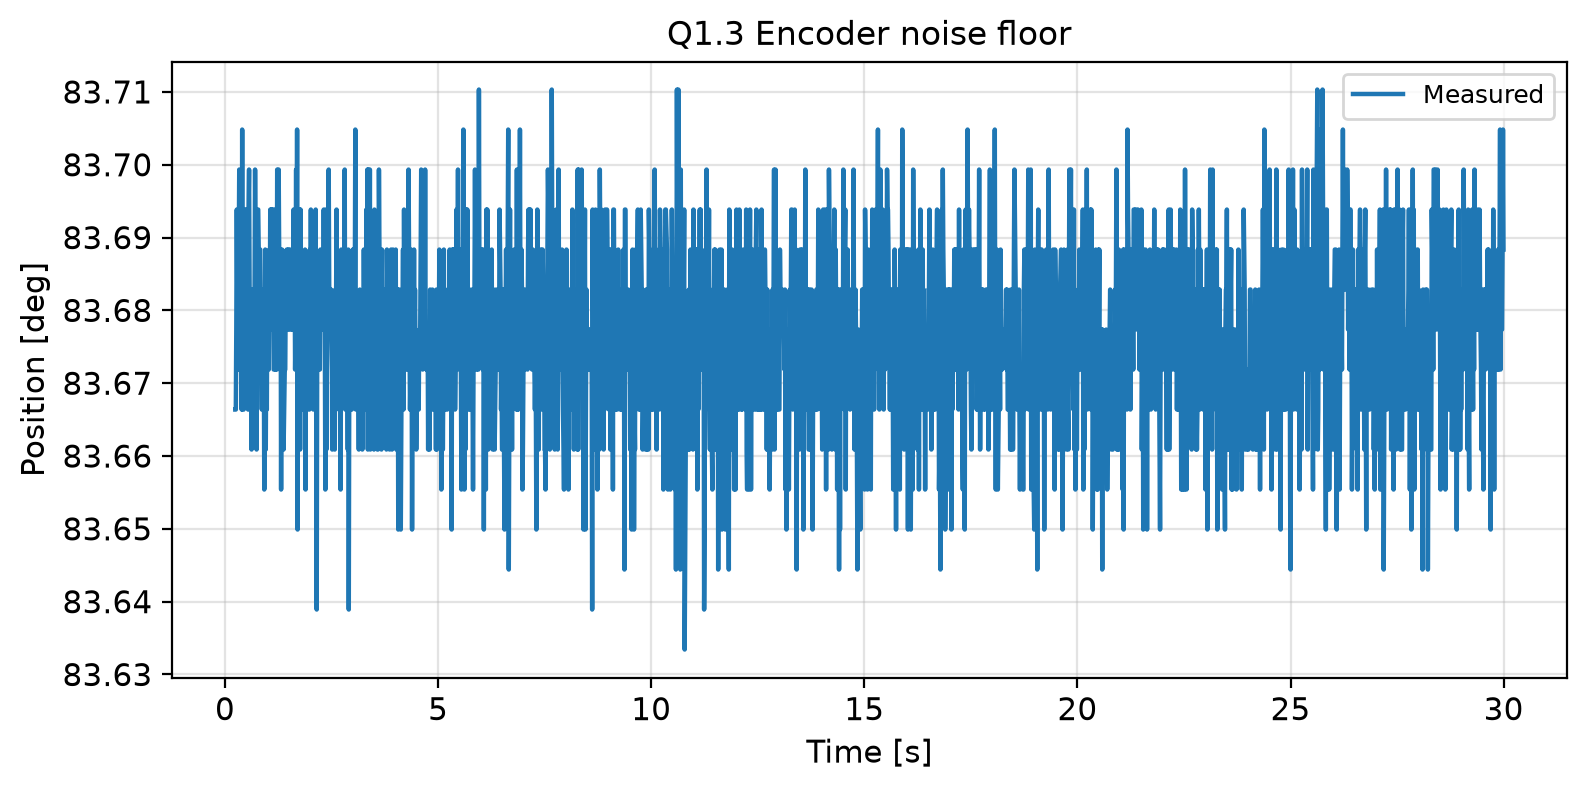
\includegraphics[width=1\textwidth]{Plots/section1_3_encoder_noise.png}
  \caption{Encoder position with the controller stopped and the shaft
  untouched.}
  \label{fig:q13}
\end{figure}

\begin{table}[H]
\centering
\caption{Encoder noise floor.}
\begin{tabular}{lll}
\toprule
 & Counts & Degrees \\
\midrule
Standard deviation & 0.5339 &  \\
Peak-to-peak       &  & 0.0769 \\
One count (quantum)& 1 &  \\
\bottomrule
\end{tabular}
\end{table}

% ANSWER: propagation discussion. Cover at least differentiation by the D term,
% noise-driven torque and heating, the quantisation deadband, and the ceiling
% it puts on usable loop gain. Forward-reference Q5.3.

% ============================================================
\section{Motor Constants}
% ============================================================

\question{P2.1}{Start from a power balance between the electrical and
mechanical ports of an ideal motor. Derive the relationship between the torque
constant in \si{\newton\meter\per\ampere} and the velocity constant in
\si{rpm\per\volt}. State every assumption you make.}

\begin{prediction}
% DERIVATION
\begin{align*}
  e\,i &= T\,\omega \\
  K_e\,\omega\,i &= K_t\,i\,\omega \\
  \Rightarrow\quad K_t\,[\si{\newton\meter\per\ampere}]
    &= K_e\,[\si{\volt\second\per\radian}]
     = \frac{60}{2\pi K_v} = \frac{9.5493}{K_v}
\end{align*}
% ASSUMPTIONS: enumerate them. Lossless, steady state, i_d = 0, sinusoidal
% back-EMF and commutation, magnetically linear, non-salient, no field
% weakening, and consistent phase/line and peak/RMS conventions.
\end{prediction}

\question{Q2.1}{Your calibration output reports a measured $K_v$, or a quantity
you can get $K_v$ from. Report it and the $K_t$ that follows. How far off is it
from the published value for this motor, as a percentage?}

\solution

\begin{table}[H]
\centering
\caption{Velocity and torque constants from calibration versus datasheet.}
\begin{tabular}{llll}
\toprule
 & Calibration & Datasheet & Difference \\
\midrule
$K_v$ (\si{rpm\per\volt}) &  & 330 &  \\
$K_t$ (\si{\newton\meter\per\ampere}) &  &  &  \\
\bottomrule
\end{tabular}
\end{table}

\question{Q2.2}{Plot torque against commanded $q$-axis current for both the
rising and the falling sweep. Fit a line to each. Report the slope as your
measured $K_t$, and report the intercept. A nonzero intercept means something
physical is happening. What is it? Does the sign make sense?}

\solution

\begin{table}[H]
\centering
\caption{Lever-arm measurement at $r = \SI{80}{\milli\meter}$.}
\begin{tabular}{lrr}
\toprule
$i_q$ (\si{\ampere}) & Rising (\si{\gram}) & Falling (\si{\gram}) \\
\midrule
1.0 & 33.6  & 37.9\\
1.5 & 49.4  & 56.7\\
2.0 & 65.3  & 72.7\\
2.5 & 85.6  & 88.6\\
3.0 & 97.7  & 104.2\\
3.5 & 113.8 & 119.9\\
4.0 & 130.2 & 134.6\\
4.5 & 146.5 & 149.4\\
5.0 & 163.0 & 163.7\\
\bottomrule
\end{tabular}
\end{table}

\begin{figure}[H]
  \centering
  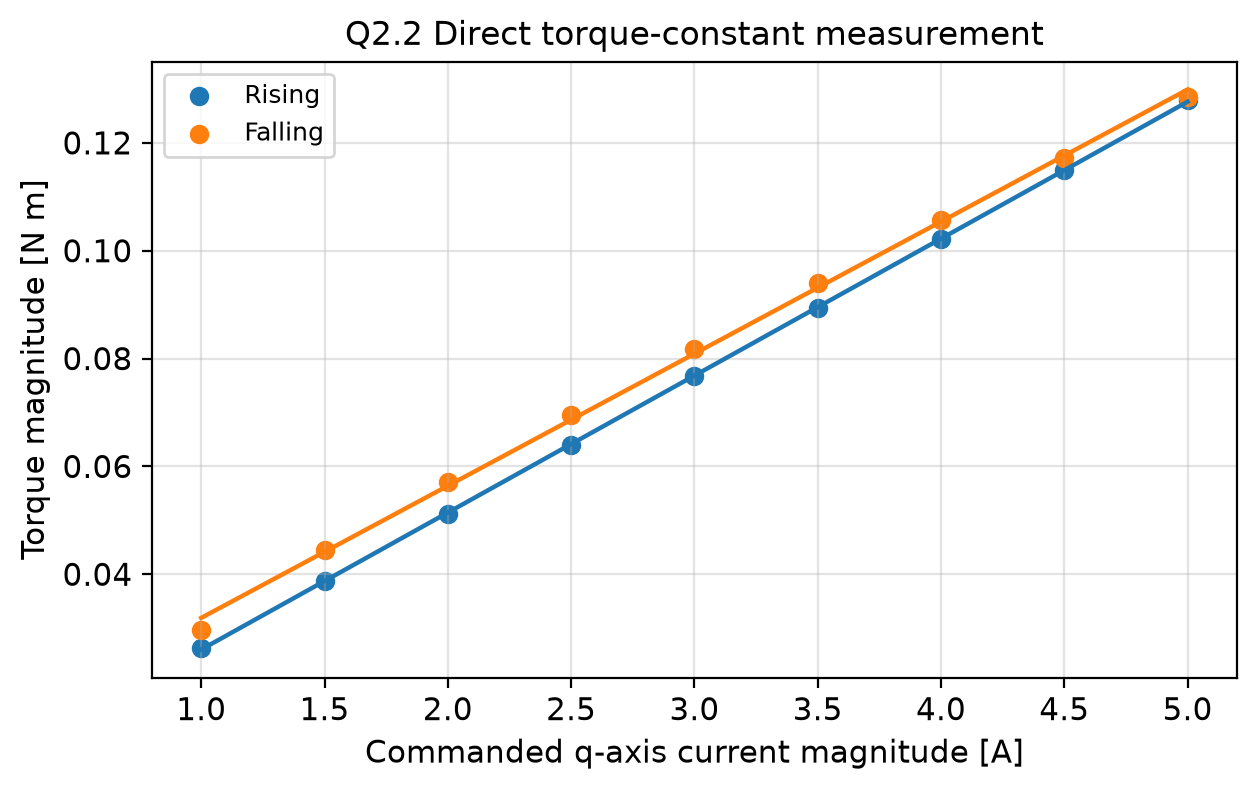
\includegraphics[width=0.8\textwidth]{Plots/section2_3_direct_measurement.png}
  \caption{Torque against commanded $q$-axis current, both sweeps, with linear
  fits extended to $i_q = 0$ so the intercepts are visible.}
  \label{fig:q22}
\end{figure}

\begin{table}[H]
\centering
\caption{Linear fits of torque against $i_q$.}
\begin{tabular}{lrr}
\toprule
Sweep & Slope $K_t$ (\si{\newton\meter\per\ampere}) & Intercept (\si{\newton\meter}) \\
\midrule
Rising &  &  \\
Falling &  &  \\
\bottomrule
\end{tabular}
\end{table}

% ANSWER: two slopes, two intercepts, the friction interpretation, and the
% sign argument. Note that the two intercepts should be equal and opposite
% about the true zero, and that half their difference is the friction torque.

\question{Q2.3}{Use your measured $K_t$ to compute the peak torque this
controller can get out of this motor within the stated limits. Explain the gap.
What would have to change to reach the advertised figure? Is that a motor
problem or a controller problem?}

\solution

\begin{table}[H]
\centering
\caption{Peak torque within controller limits versus advertised motor peak.}
\begin{tabular}{ll}
\toprule
Quantity & Value \\
\midrule
Measured $K_t$ &  \\
Controller peak current & \SI{20}{\ampere} \\
Implied peak torque &  \\
Advertised peak torque & \SI{1.7}{\newton\meter} \\
\bottomrule
\end{tabular}
\end{table}

% ============================================================
\section{Commutation}
% ============================================================

\question{Q3.1}{The \texttt{d pwm} command takes an angle and a voltage
magnitude. Work out the units of the angle from your own sweep. Is the angle in
degrees or in radians? Is it a mechanical angle or an electrical one? What in
your data settles it?}

\solution

% ANSWER: give the competing hypotheses and what each predicts, then the data.

\question{Q3.2}{Plot mechanical rotor angle against commanded electrical phase.
Report the slope and extract the number of pole pairs. How does that compare
with the pole count from Q1.1?}

\solution

\begin{figure}[H]
  \centering
  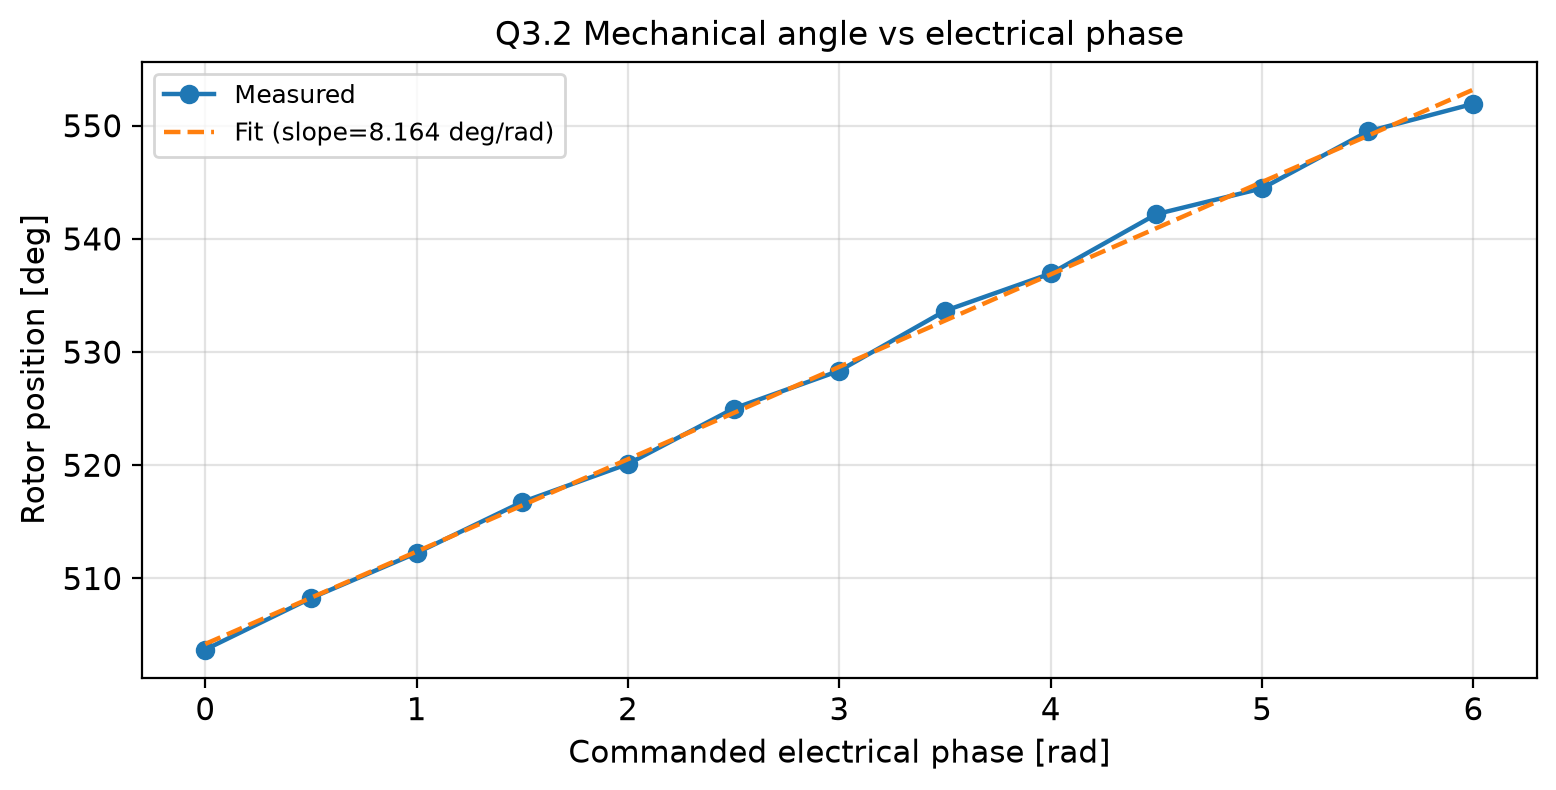
\includegraphics[width=0.8\textwidth]{Plots/section3_1_phase_sweep.png}
  \caption{Mechanical rotor angle against commanded electrical phase, unwrapped,
  with linear fit.}
  \label{fig:q32}
\end{figure}

\begin{equation*}
  \theta_{\text{mech}} = \frac{1}{p}\,\theta_{\text{elec}}
  \qquad\Rightarrow\qquad p = \frac{1}{\text{slope}}
\end{equation*}

% ANSWER.

\question{P3.1}{Before you run anything, predict what the shaft does under each
of the three commands. What will $i_d$ and $i_q$ read once each one has settled?}

\begin{prediction}
prediction for 3.1
\end{prediction}

\question{Q3.3}{Run all three commands at the same current magnitude. Report the
measured $i_d$ and $i_q$ in each case. Which command produces torque, and which
does not? For the case that produced no torque: where is the power going?}

\solution

\begin{table}[H]
\centering
\caption{Settled $i_d$ and $i_q$ for the three Park-transform commands.}
\begin{tabular}{lrr}
\toprule
Command & $i_d$ (\si{\ampere}) & $i_q$ (\si{\ampere}) \\
\midrule
\texttt{d pwm} &  &  \\
\texttt{d dq 0 $I$} &  &  \\
\texttt{d dq $I$ 0} &  &  \\
\bottomrule
\end{tabular}
\end{table}

\begin{figure}[H]
  \centering
  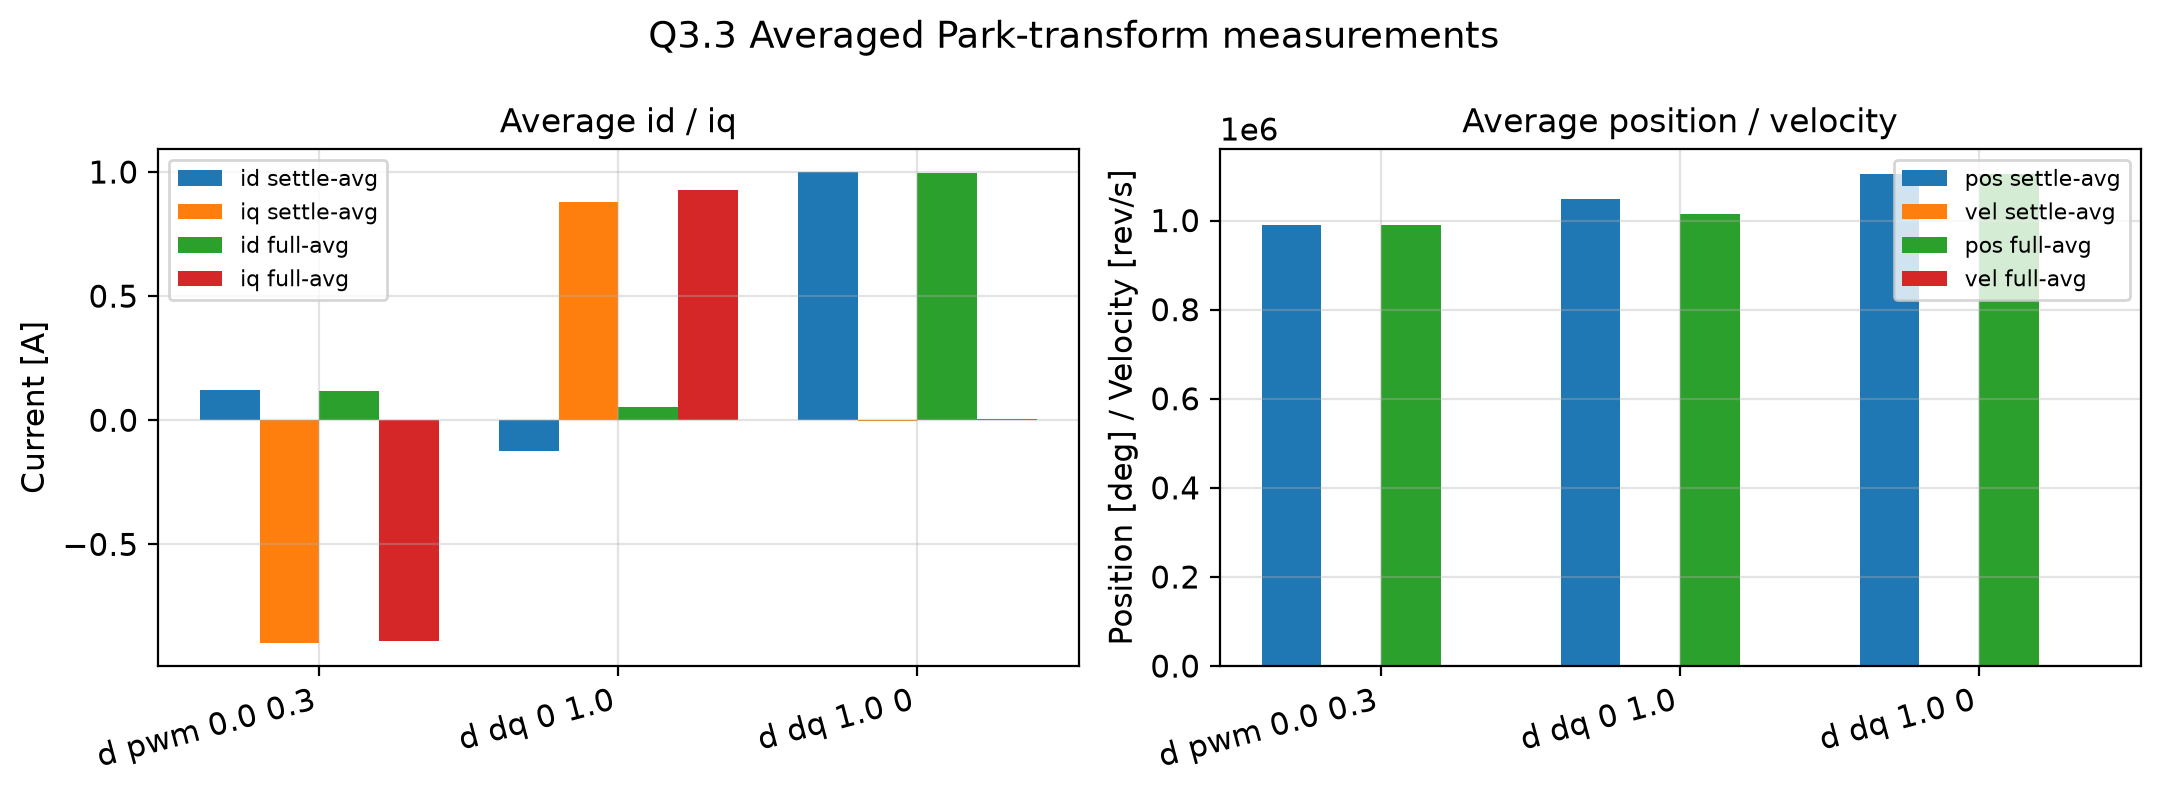
\includegraphics[width=0.9\textwidth]{Plots/section3_2_park_transform_averages.png}
  \caption{Measured $d$- and $q$-axis currents for \texttt{d pwm}, \texttt{d dq}
  $0\,I$, and \texttt{d dq} $I\,0$.}
  \label{fig:q33}
\end{figure}

% ============================================================
\section{The Command Protocol}
% ============================================================

\question{Q4.1}{Decode the frame \texttt{8002 01000A0D200000C07F11001F01130D50}
completely. Give a table with one row per field: byte offset, raw bytes,
meaning, and decoded value in engineering units. Account for every byte,
including the padding. What does the 8 in \texttt{8002} do? What does the 2 do?}

\solution

\subsection*{Payload}
 
\begin{table}[H]
\centering
\caption{Decode of the \SI{16}{\byte} command payload. Every byte accounted for.}
\small
\setlength{\extrarowheight}{5pt}%
\begin{tabular}{|p{1.1cm}|p{2.2cm}|p{3.0cm}|p{6.0cm}|p{1.3cm}|}
\hline
\textbf{Byte offset} & \textbf{Raw bytes} & \textbf{Meaning} &
\textbf{Decoded value} & \textbf{Unit} \\
\hline
 
0 & \texttt{01} & Opcode: write 1 consecutive int8 register &
\opcell{01}{0000}{00}{01}
   {write\\operation}{int8\\data type}{1 register} & --- \\[0.4em] \hline
 
1 & \texttt{00} & Target address & Register \texttt{0x000} $\rightarrow$ Mode register
& --- \\[0.4em] \hline
 
2 & \texttt{0A} & Value & $(\text{0A})_{16} = (10)_{10}$ $\rightarrow$ Position mode
& --- \\[0.4em] \hline
 
3 & \texttt{0D} & Opcode: write 1 float register &
\opcell{0D}{0000}{11}{01}
   {write\\operation}{float\\data type}{1 register} & --- \\[0.4em] \hline
 
4 & \texttt{20} & Target address & Register \texttt{0x020} $\rightarrow$ command position
& --- \\[0.4em] \hline
 
5--8 & \texttt{00 00 C0 7F} & Value (float, \SI{4}{\byte}) &
Little-endian, so reverse to \texttt{0x7FC00000}. Exponent all ones with a
nonzero mantissa $\Rightarrow$ \textbf{NaN} & rev \\[0.4em] \hline
 
9 & \texttt{11} & Opcode: read 1 int8 register &
\opcell{11}{0001}{00}{01}
   {read\\operation}{int8\\data type}{1 register} & --- \\[0.4em] \hline
 
10 & \texttt{00} & Target address & Register \texttt{0x000} $\rightarrow$ reading Mode
& --- \\[0.4em] \hline
 
11 & \texttt{1F} & Opcode: read 3 consecutive float registers &
\opcell{1F}{0001}{11}{11}
   {read\\operation}{float\\data type}{3 registers} & --- \\[0.4em] \hline
 
12 & \texttt{01} & Target address &
Starting from \texttt{0x001}:
\texttt{0x001} position,
\texttt{0x002} velocity,
\texttt{0x003} torque &
rev, rev/s, \si{\newton\meter} \\[0.4em] \hline
 
13 & \texttt{13} & Opcode: read 3 consecutive int8 registers &
\opcell{13}{0001}{00}{11}
   {read\\operation}{int8\\data type}{3 registers} & --- \\[0.4em] \hline
 
14 & \texttt{0D} & Target address &
Starting from \texttt{0x00D}:
\texttt{0x00D} voltage,
\texttt{0x00E} temperature,
\texttt{0x00F} fault code &
\si{\volt}, \si{\celsius}, --- \\[0.4em] \hline
 
15 & \texttt{50} & \texttt{nop} & Padding & --- \\ \hline

\multicolumn{5}{|l|}{\textbf{Total: \SI{16}{\byte}}} \\
\hline
\end{tabular}
\end{table}


\subsection*{Arbitration ID}
 
\texttt{8002} is the 16-bit CAN ID, formed as
\texttt{(source\,\textless\textless\,8)\,|\,destination}, with the most
significant bit set when a reply is requested.
 
\begin{table}[H]
\centering
\caption{Arbitration ID fields for \texttt{8002}.}
\begin{tabular}{lll}
\hline
Field & Value & Meaning \\
\hline
Bit 15 (the \texttt{8}) & 1 & Reply requested \\
Source  & \texttt{0x00} & Host \\
Destination (the \texttt{2}) & \texttt{0x02} & Controller, node 2 \\
\hline
\end{tabular}
\end{table}
 
\subsection*{On the padding}
 
All useful data ends at byte 14, giving \SI{15}{\byte}. CAN-FD payload lengths
are quantised --- 0 to 8, then 12, 16, 20, 24, 32, 48 and \SI{64}{\byte} --- and
there is no legal length of 15. One \texttt{nop} byte rounds the frame up to
\SI{16}{\byte}.
 
\subsection*{On frame density}
 
Subframes at offsets 9, 11 and 13 are read requests. A read supplies no value,
so it carries no data bytes, and all three requests together occupy only
\SI{6}{\byte}. By contrast the single float write at offset 3 occupies
\SI{6}{\byte} on its own. The frame therefore performs five separate operations
in \SI{16}{\byte}: it sets the mode, commands a position, and queues three
independent read-backs.
 

% ANSWER: the two ID questions, and the padding reason (legal CAN-FD lengths).

\question{Q4.2}{Decode the reply on the following line. Report position,
velocity, torque, bus voltage, board temperature, and fault code in engineering
units. One of those values tells you something about the bench that this handout
never states. Which value is it? What does it tell you?}

\solution

The reply arrives with CAN ID \texttt{0x0200}: source \texttt{0x02}
(the controller), destination \texttt{0x00} (the host), reply bit clear.
Byte offsets below are numbered from the start of this frame.

\begin{table}[H]
\centering
\caption{Decode of the \SI{24}{\byte} reply payload.}
\small
\setlength{\extrarowheight}{5pt}%
\begin{tabular}{|p{1.1cm}|p{2.2cm}|p{2.8cm}|p{6.2cm}|p{1.3cm}|}
\hline
\textbf{Byte offset} & \textbf{Raw bytes} & \textbf{Meaning} &
\textbf{Decoded value} & \textbf{Unit} \\
\hline

0 & \texttt{21} & Opcode: reply, 1 int8 register &
\opcell{21}{0010}{00}{01}
   {reply\\operation}{int8\\data type}{1 register} & --- \\[0.4em] \hline

1 & \texttt{00} & Target address & Register \texttt{0x000} $\rightarrow$ Mode
& --- \\[0.4em] \hline

2 & \texttt{00} & Value & $(\text{00})_{16} = 0$ $\rightarrow$ Stopped & --- \\[0.4em] \hline

3 & \texttt{2F} & Opcode: reply, 3 float registers &
\opcell{2F}{0010}{11}{11}
   {reply\\operation}{float\\data type}{3 registers} & --- \\[0.4em] \hline

4 & \texttt{01} & Target address &
Starting from \texttt{0x001}, 3 registers & --- \\[0.4em] \hline

5--8 & \texttt{00 28 26 40} & Position (float) &
See derivation below: \textbf{2.596191} & rev \\[0.4em] \hline

9--12 & \texttt{FC A6 64 BC} & Velocity (float) &
See derivation below: \textbf{$-0.013956$} & rev/s \\[0.4em] \hline

13--16 & \texttt{00 00 00 00} & Torque (float) &
All bits zero $\rightarrow$ the reserved pattern for exactly \textbf{0} &
\si{\newton\meter} \\[0.4em] \hline

17 & \texttt{23} & Opcode: reply, 3 int8 registers &
\opcell{23}{0010}{00}{11}
   {reply\\operation}{int8\\data type}{3 registers} & --- \\[0.4em] \hline

18 & \texttt{0D} & Target address &
Starting from \texttt{0x00D}, 3 registers & --- \\[0.4em] \hline

19 & \texttt{30} & Bus voltage &
$(\text{30})_{16} = (48)_{10}$, scale \SI{0.5}{\volt\per\lsb}
$\Rightarrow$ \textbf{24.0} & \si{\volt} \\[0.4em] \hline

20 & \texttt{1F} & Board temperature &
$(\text{1F})_{16} = (31)_{10}$, scale \SI{1}{\celsius\per\lsb}
$\Rightarrow$ \textbf{31} & \si{\celsius} \\[0.4em] \hline

21 & \texttt{00} & Fault code & \textbf{0} $\rightarrow$ no fault & --- \\[0.4em] \hline

22--23 & \texttt{50 50} & \texttt{nop} $\times$ 2 &
Padding, \SI{22}{\byte} $\rightarrow$ \SI{24}{\byte} & --- \\ \hline

\multicolumn{5}{|l|}{\textbf{Total: \SI{24}{\byte}}} \\
\hline
\end{tabular}
\end{table}

\subsection*{Float derivations}

\paragraph{Position, bytes 5--8.}
Wire order \texttt{00 28 26 40}; reversed for little-endian this is
\texttt{0x40262800}.

\begin{center}
\setlength{\tabcolsep}{10pt}%
\begin{tabular}{ccc}
\underline{\texttt{0}} &
\underline{\texttt{1000 0000}} &
\underline{\texttt{010 0110 0010 1000 0000 0000}} \\[0.2em]
\scriptsize sign & \scriptsize exponent & \scriptsize mantissa
\end{tabular}
\end{center}

\begin{align*}
  \text{sign}     &= 0 \\
  \text{exponent} &= (1000\,0000)_2 = 128 \\
  \text{mantissa} &= (\text{0x262800})_{16} = 2\,500\,608
\end{align*}

\begin{align*}
  \text{value} &= (-1)^{\text{sign}}
     \left(1 + \frac{\text{mantissa}}{2^{23}}\right) 2^{\,\text{exponent}-127} \\
   &= (+1)\left(1 + \frac{2\,500\,608}{8\,388\,608}\right) 2^{\,128-127} \\
   &= 1.298096 \times 2 = \SI{2.596191}{\rev}
\end{align*}

\paragraph{Velocity, bytes 9--12.}
Wire order \texttt{FC A6 64 BC}; reversed this is \texttt{0xBC64A6FC}.

\begin{center}
\setlength{\tabcolsep}{10pt}%
\begin{tabular}{ccc}
\underline{\texttt{1}} &
\underline{\texttt{0111 1000}} &
\underline{\texttt{110 0100 1010 0110 1111 1100}} \\[0.2em]
\scriptsize sign & \scriptsize exponent & \scriptsize mantissa
\end{tabular}
\end{center}

\begin{align*}
  \text{sign}     &= 1 \\
  \text{exponent} &= (0111\,1000)_2 = 120 \\
  \text{mantissa} &= (\text{0x64A6FC})_{16} = 6\,596\,348
\end{align*}

\begin{align*}
  \text{value} &= (-1)^{\text{sign}}
     \left(1 + \frac{\text{mantissa}}{2^{23}}\right) 2^{\,\text{exponent}-127} \\
   &= (-1)^{1}\left(1 + \frac{6\,596\,348}{8\,388\,608}\right) 2^{\,120-127} \\
   &= -1.786346 \times 2^{-7} = \SI{-0.013956}{\rev\per\second}
\end{align*}

\paragraph{Torque, bytes 13--16.} All thirty-two bits are zero, which is the
reserved IEEE-754 pattern for exactly zero rather than a value obtained from the
normal formula. Torque $= \SI{0}{\newton\meter}$, consistent with mode 0: the
output stage is off, so no current flows and no torque is commanded.

\subsection*{What the reply says about the bench}

% ANSWER THIS - second half of the question.

\question{Q4.3}{The position value in that command frame is a floating point
NaN. What does the controller do with it? Why is being able to send NaN useful?
Give a situation where you would want it.}

\solution

% ANSWER.

\question{Q4.4}{Count the bytes in the long command frame. Estimate the highest
rate at which you could command one motor and read its state back, first using
float resolution and then using int16. State your assumptions. Did you count the
reply as well as the command? Compare both numbers against \SI{1}{\kilo\hertz}
and against the sample rate you achieved in Q1.3. Which of the two is the real
limit in this lab?}

\solution

\paragraph{Assumptions.}
\begin{enumerate}\itemsep0em
  \item % bit rate
  \item % overhead per frame
  \item % command plus reply counted
  \item % bus otherwise idle
\end{enumerate}

\begin{equation*}
  t_{\text{frame}} = \frac{8N + 30}{R_{\text{bit}}}, \qquad
  f_{\max} = \frac{1}{t_{\text{cmd}} + t_{\text{reply}}}
\end{equation*}

\begin{table}[H]
\centering
\caption{Achievable command rate.}
\begin{tabular}{lrrrr}
\hline
Encoding & Cmd (\si{\byte}) & Reply (\si{\byte}) & Round trip & Rate \\
\hline
float &  &  &  &  \\
int16 &  &  &  &  \\
\hline
\end{tabular}
\end{table}

% ANSWER: the comparison, including the observed round trips in the capture's
% own timestamps and your Q1.3 rate. Note the int16 position range limit.

% ============================================================
\section{Position Control and Step Response}
% ============================================================

\question{P5.1}{With $k_d$ and $k_i$ zero, predict what you will feel when you
displace the shaft by hand and release it. As you raise $k_p$, what will
eventually go wrong? Name the mechanical component the motor is imitating when
only $k_p$ is set.}

\begin{prediction}
% ANSWER. Predict a mechanism, not just an outcome.
\end{prediction}

\question{Q5.1}{Report the $k_p$ at which it went unstable, and the value you
backed off to. Log position while it is misbehaving, and include the plot.
Describe what the instability sounds and feels like. What do you think set the
limit?}

\solution

\begin{figure}[H]
  \centering
  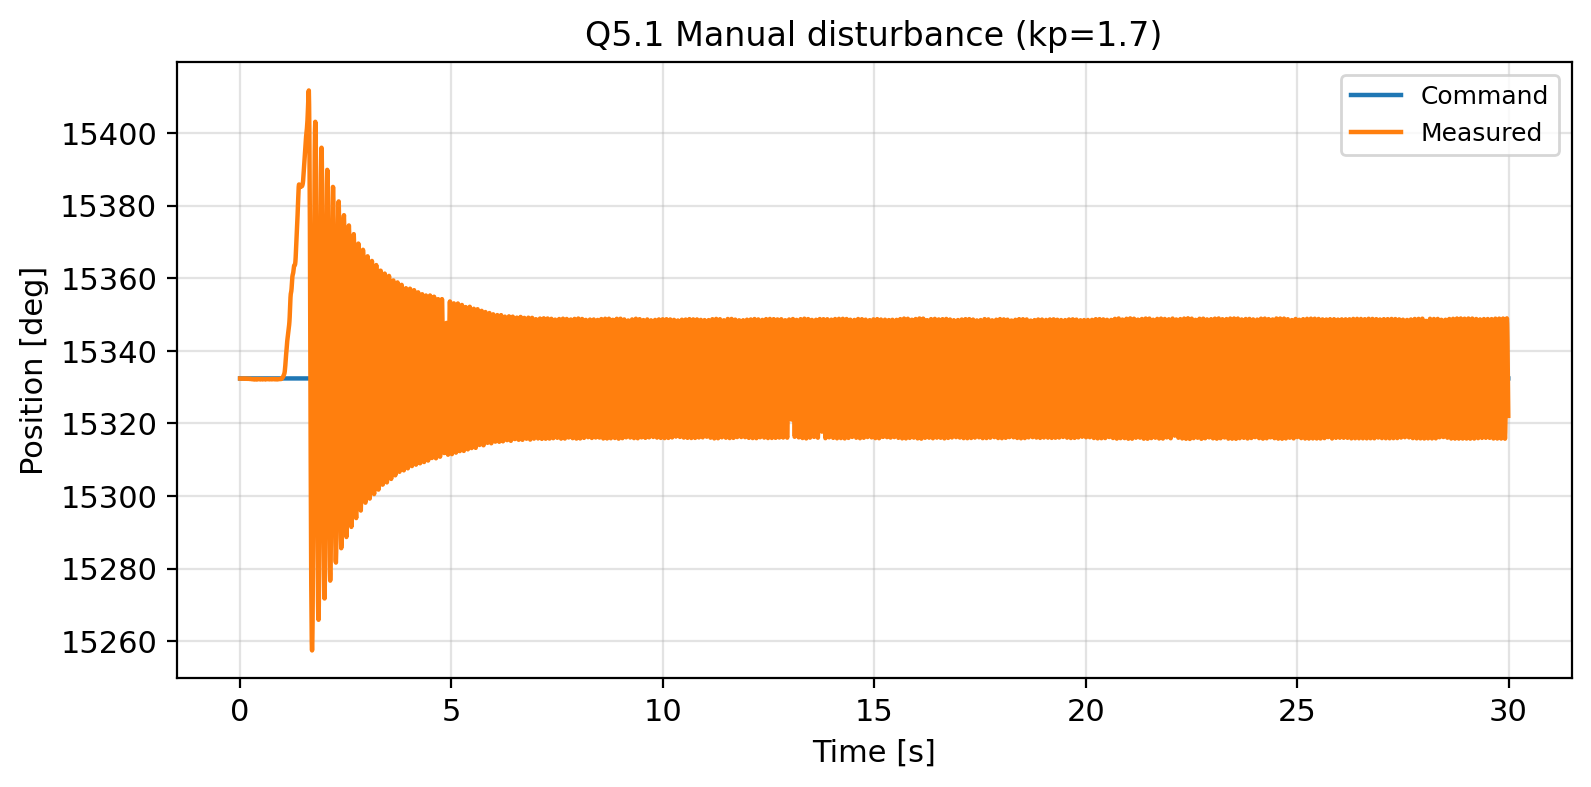
\includegraphics[width=0.85\textwidth]{Plots/section5_1_hold_disturbance.png}
  \caption{Logged position at the onset of instability.}
  \label{fig:q51}
\end{figure}

% ANSWER. Include the measured oscillation frequency and use it to argue which
% mechanism set the limit.

\question{Q5.2}{Displace the shaft by hand and release. Then command a small
position step. Plot both. Describe the response and compare against your P5.1
prediction. If it does not ring the way you predicted, why not?}

\solution

\begin{figure}[H]
  \centering
  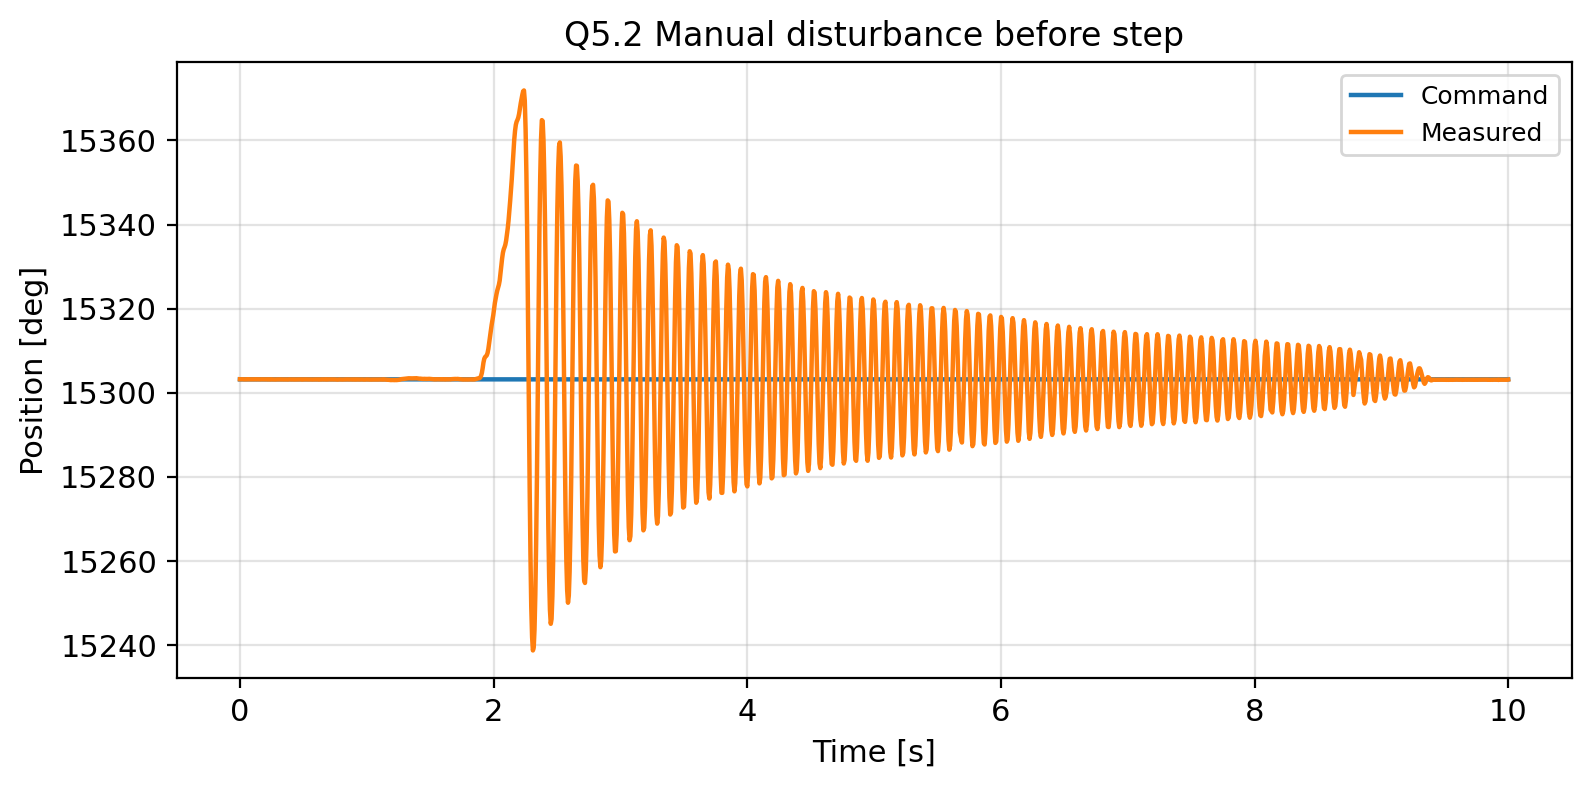
\includegraphics[width=0.85\textwidth]{Plots/section5_2_hold_disturbance.png}
  \caption{Displace-and-release with $k_d = 0$.}
  \label{fig:q52a}
\end{figure}

\begin{figure}[H]
  \centering
  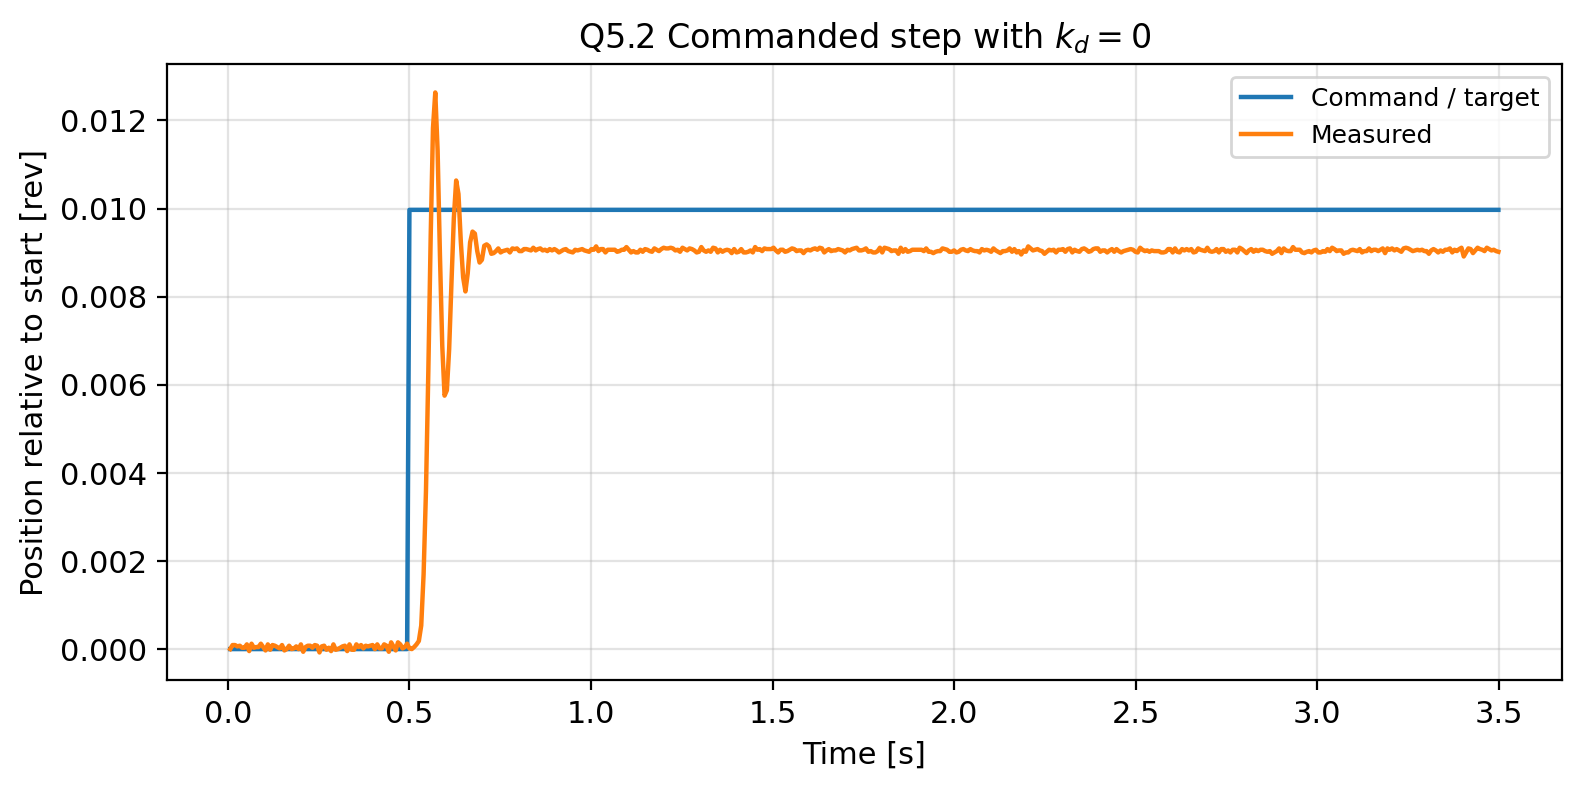
\includegraphics[width=0.85\textwidth]{Plots/section5_1_step.png}
  \caption{Commanded step with $k_d = 0$.}
  \label{fig:q52b}
\end{figure}

% ANSWER. Link the park-short error to the friction torque measured in Q2.2:
% e_deadband = T_friction / k_p.

\question{Q5.3}{Raise $k_d$ until the step response is critically damped, with
just barely no overshoot. Report your final $k_p$ and $k_d$, and plot that step
response. Then keep raising $k_d$ past that point. What goes wrong? What is
causing this problem?}

\solution

\begin{table}[H]
\centering
\caption{Final gains.}
\begin{tabular}{lll}
\toprule
 & Configured & Converted (per radian) \\
\midrule
$k_p$ & 1.6   & 0.254648 \\
$k_d$ & 0.075 & 0.011937 \\
\bottomrule
\end{tabular}
\end{table}

\begin{figure}[H]
  \centering
  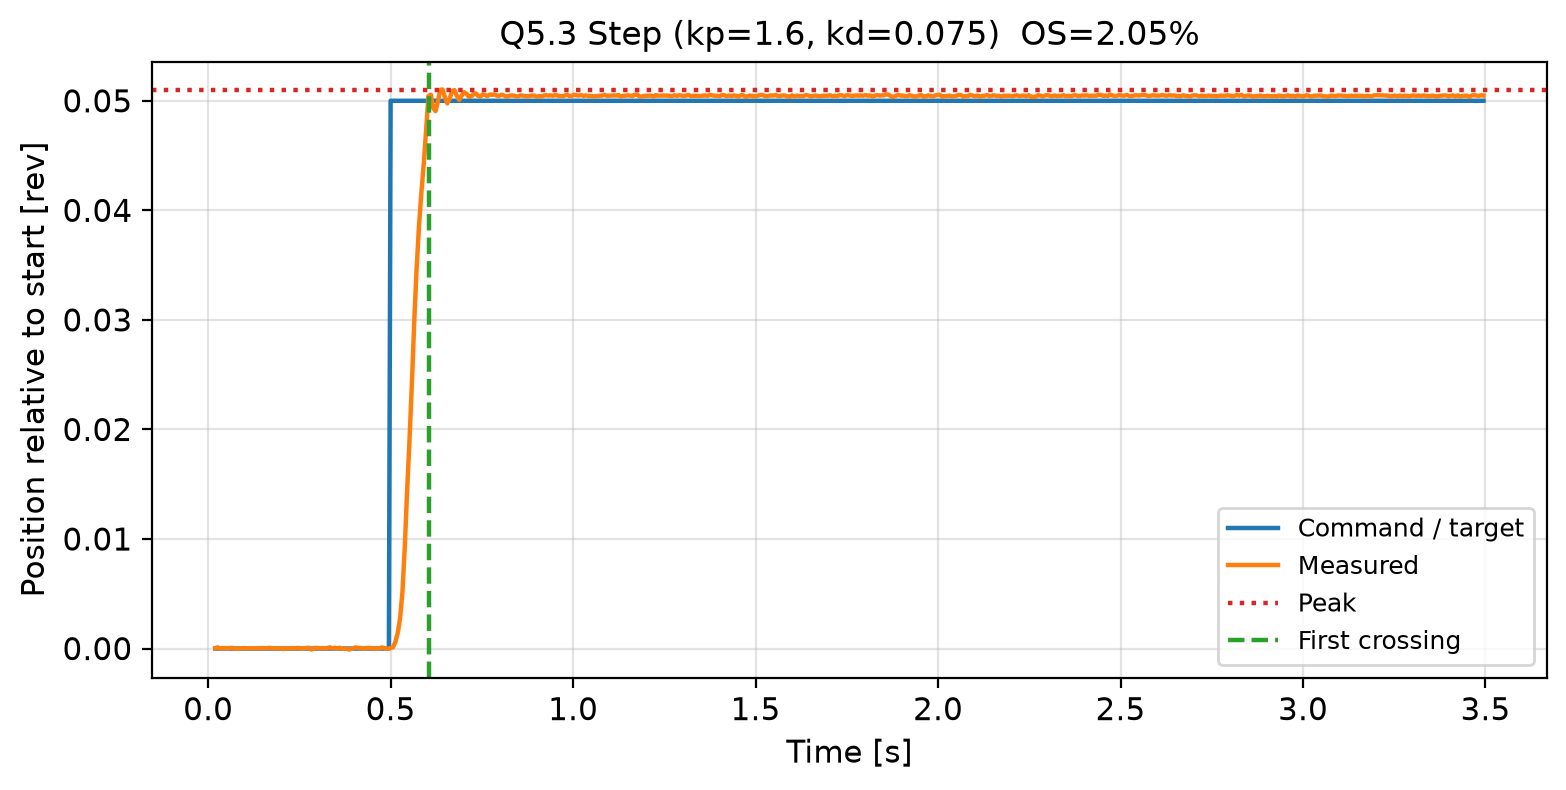
\includegraphics[width=0.85\textwidth]{Plots/section5_3_step.png}
  \caption{Step response at the final gains, step size \SI{0.05}{\rev}.}
  \label{fig:q53}
\end{figure}

\begin{figure}[H]
  \centering
  \includegraphics[width=0.85\textwidth]{Plots/section5_3_kd_too_high.png}
  \caption{Step response with $k_d$ raised past critical damping.}
  \label{fig:q53b}
\end{figure}

% ANSWER: what breaks at high k_d, and the mechanism. Make the noise argument
% quantitative using sigma from Q1.3 and your sample rate.

\paragraph{Choosing $k_i$ and ilimit.}
\begin{equation*}
  I_e = \int_0^{t_1}\! e(t)\,dt, \qquad
  k_i \approx \frac{0.1\,k_p e_0}{I_e} = \frac{0.008}{I_e}, \qquad
  \text{ilimit} \gtrsim \text{few}\times k_p e_{ss}
\end{equation*}
% Report I_e, the k_i it gives, e_ss, and your chosen ilimit. State your
% stopping criterion for the integral if the response has no clean crossing.

\begin{table}[H]
\centering
\caption{Integral gain from the Q5.3 error integral.}
\begin{tabular}{ll}
\toprule
Quantity & Value \\
\midrule
$e_0$ &  \\
$I_e$ &  \\
$k_i$ &  \\
$e_{ss}$ &  \\
ilimit &  \\
\bottomrule
\end{tabular}
\end{table}

\question{Q5.4}{Set $k_i$ and ilimit to the values you worked out, then do the
three tests. Report what integral action fixed, and what it cost. The behaviour
you see when you release the held shaft has a standard name. What is it?
Compare your two releases. What is ilimit protecting you from? What does setting
it too low cost you?}

\solution

\begin{figure}[H]
  \centering
  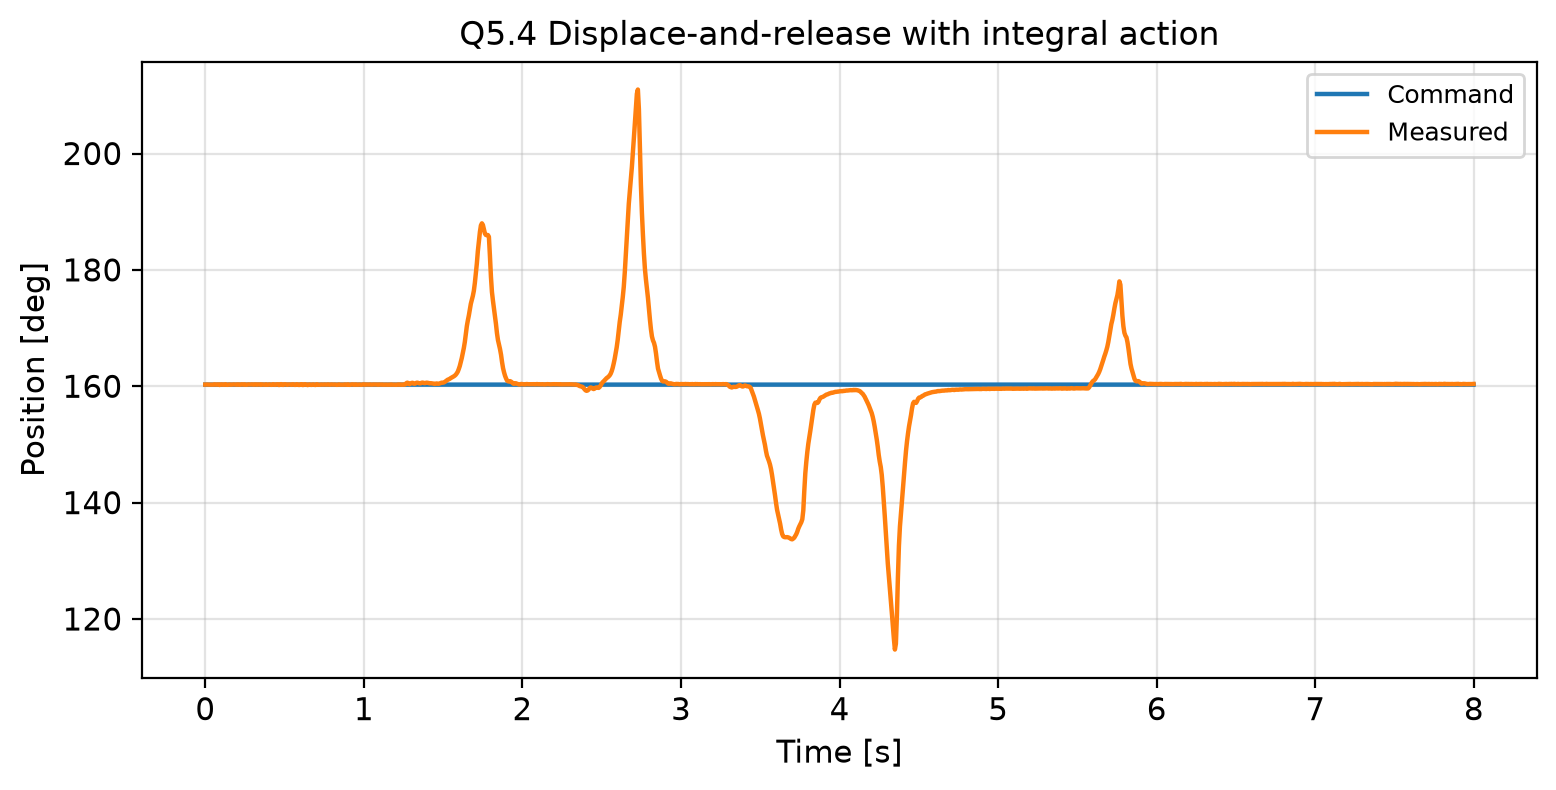
\includegraphics[width=0.85\textwidth]{Plots/section5_4_displace_release.png}
  \caption{Displace-and-release with integral action enabled.}
  \label{fig:q54a}
\end{figure}

\begin{figure}[H]
  \centering
  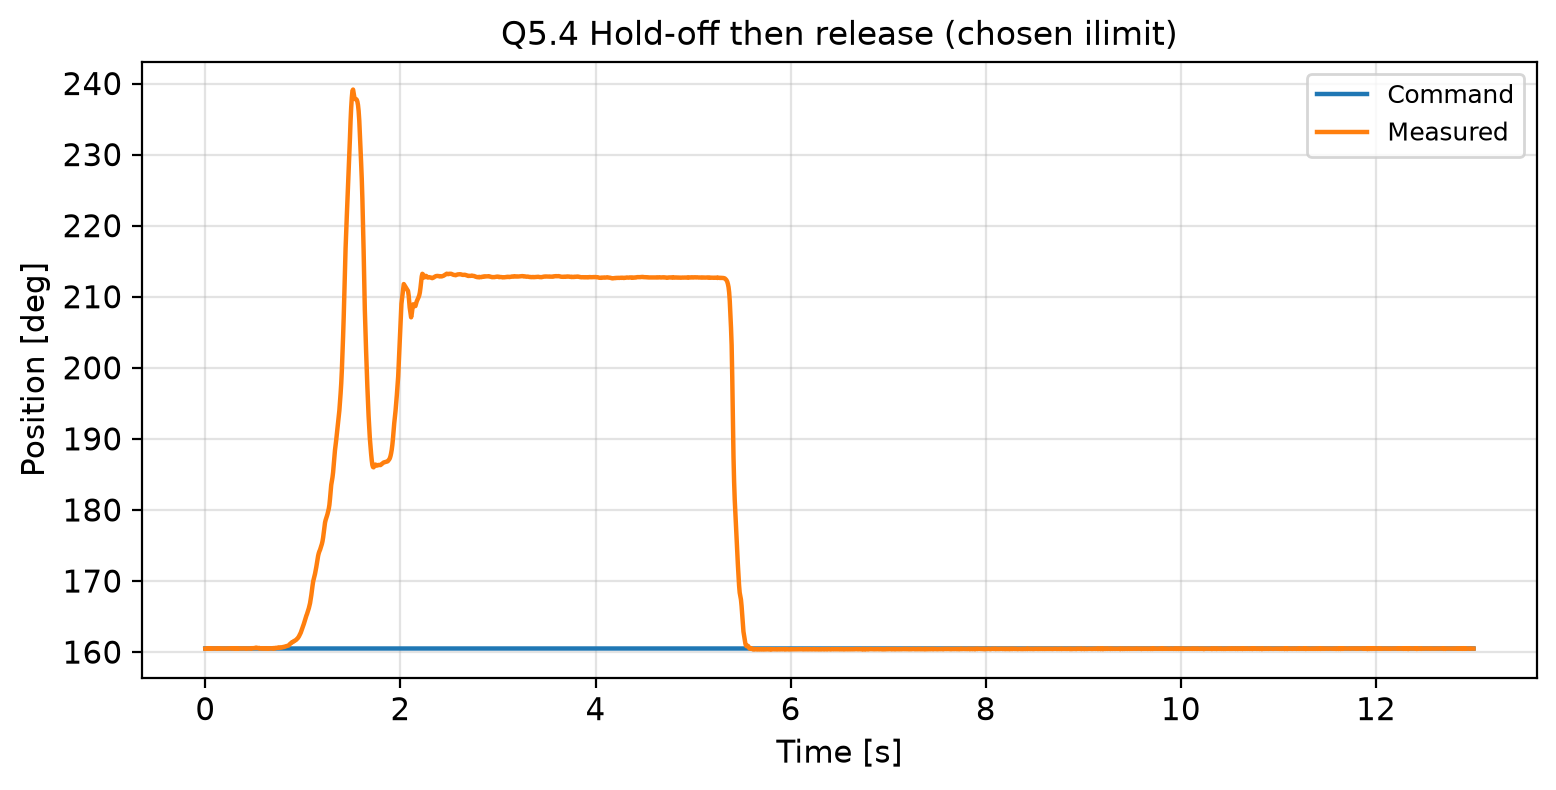
\includegraphics[width=0.85\textwidth]{Plots/section5_4_hold_release_ilimit.png}
  \caption{Release after a five-second hold \SI{20}{\degree} off target at the
  chosen ilimit.}
  \label{fig:q54b}
\end{figure}

\begin{figure}[H]
  \centering
  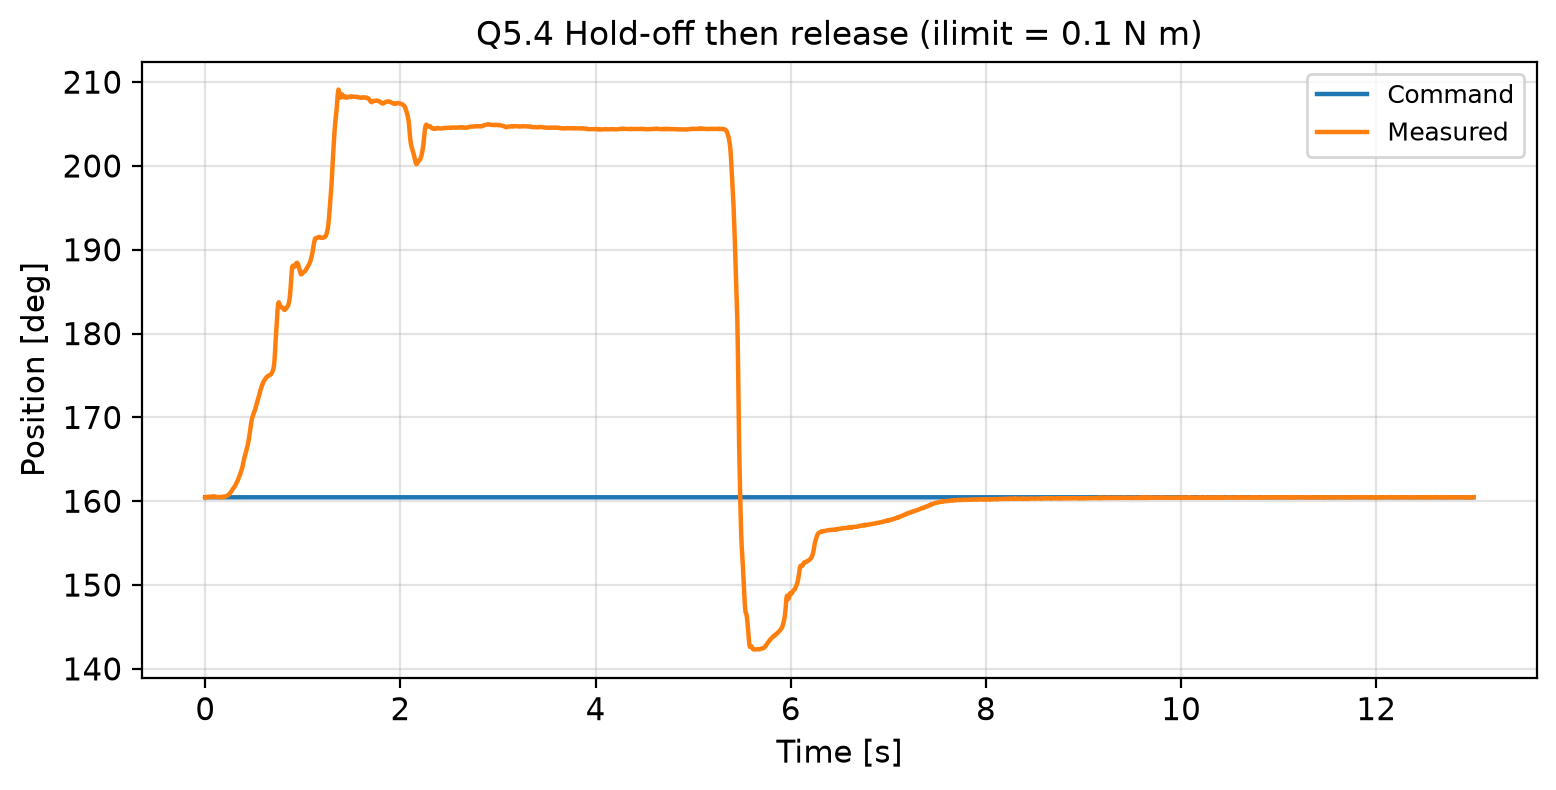
\includegraphics[width=0.85\textwidth]{Plots/section5_4_hold_release_ilimit_max.png}
  \caption{Release after a five-second hold \SI{20}{\degree} off target at
  ilimit $= \SI{0.1}{\newton\meter}$.}
  \label{fig:q54c}
\end{figure}

\begin{figure}[H]
  \centering
  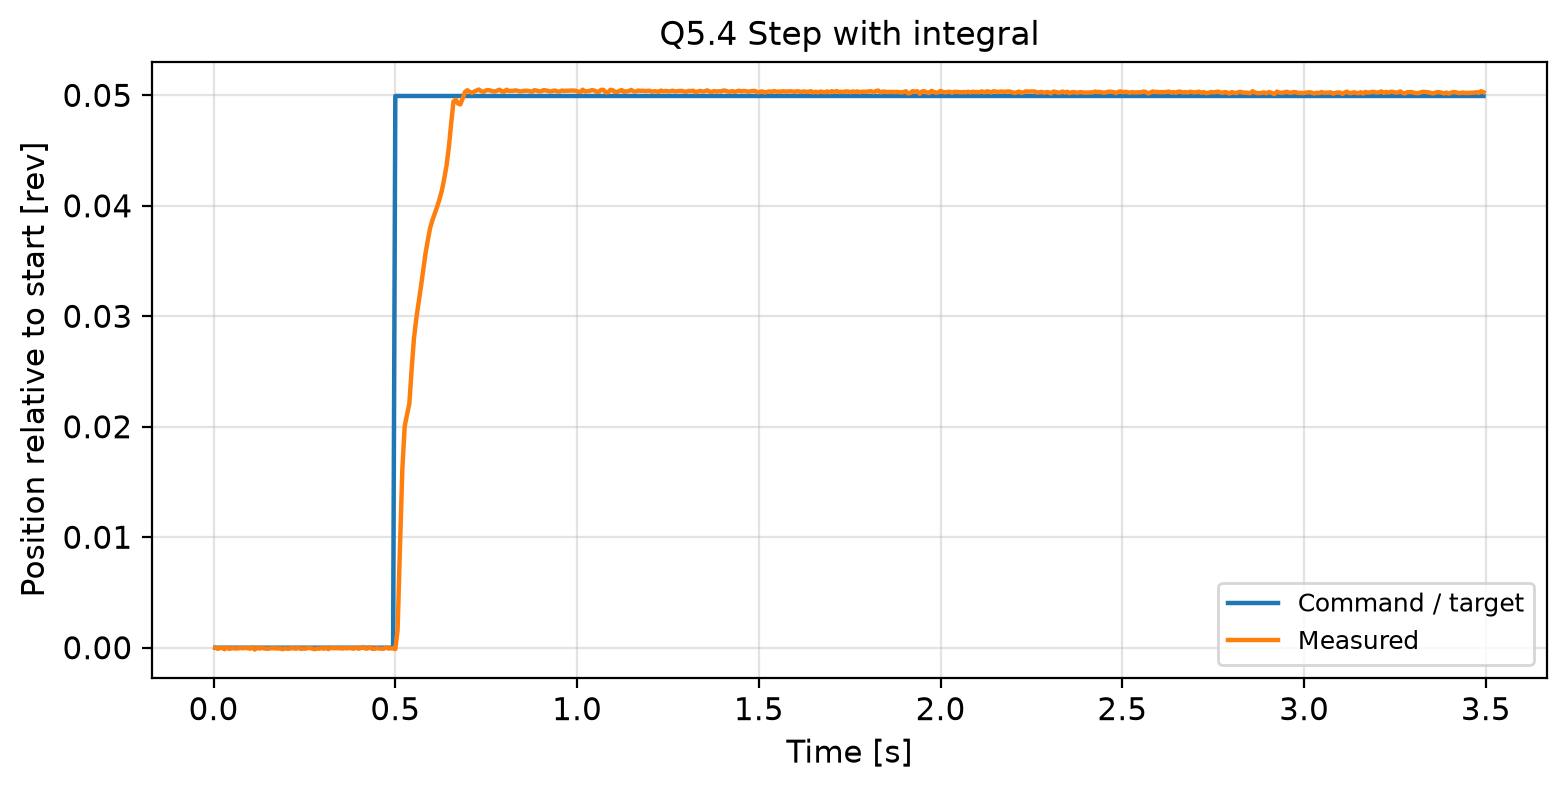
\includegraphics[width=0.85\textwidth]{Plots/section5_4_step.png}
  \caption{Step response with $k_i$ and ilimit set to the Q5.3 values.}
  \label{fig:q54d}
\end{figure}

% ANSWER. Quantify: the unclamped integral term after the hold is
% k_i * 0.0556 rev * 5 s. Compare against ilimit.

\question{Q5.5}{Take the measured overshoot and rise time at one gain setting.
Extract the damping ratio and the natural frequency, then solve for $J$. Report
this as your first estimate of rotor inertia. Then estimate the same thing with
calipers, treating the rotor as a thin steel ring.}

\solution

\begin{align*}
  \zeta &= \frac{-\ln M_p}{\sqrt{\pi^2 + \ln^2 M_p}}, &
  \omega_n &= \frac{\pi}{t_p\sqrt{1-\zeta^2}}, &
  J &= \frac{k_p^{\text{rad}}}{\omega_n^2}
\end{align*}

From the underdamped Q5.2 step ($k_p=1.6$, $k_d=0$):
$M_p = 27.1\%$, $t_p = 71.2\,\mathrm{ms}$ $\Rightarrow$
$\zeta = 0.384$, $\omega_n = 47.8\,\mathrm{rad/s}$,
$J_{\text{step}} = 1.11\times 10^{-4}\,\mathrm{kg\,m^2}$.

Caliper thin ring (steel $\rho=7800\,\mathrm{kg/m^3}$):
OD $=63\,\mathrm{mm}$, radial wall $=4\,\mathrm{mm}$ (ID $=55\,\mathrm{mm}$),
axial $=11.7\,\mathrm{mm}$ $\Rightarrow$
$J_{\text{ring}} = \tfrac12 m(R_o^2+R_i^2) = 5.92\times 10^{-5}\,\mathrm{kg\,m^2}$.

\begin{figure}[H]
  \centering
  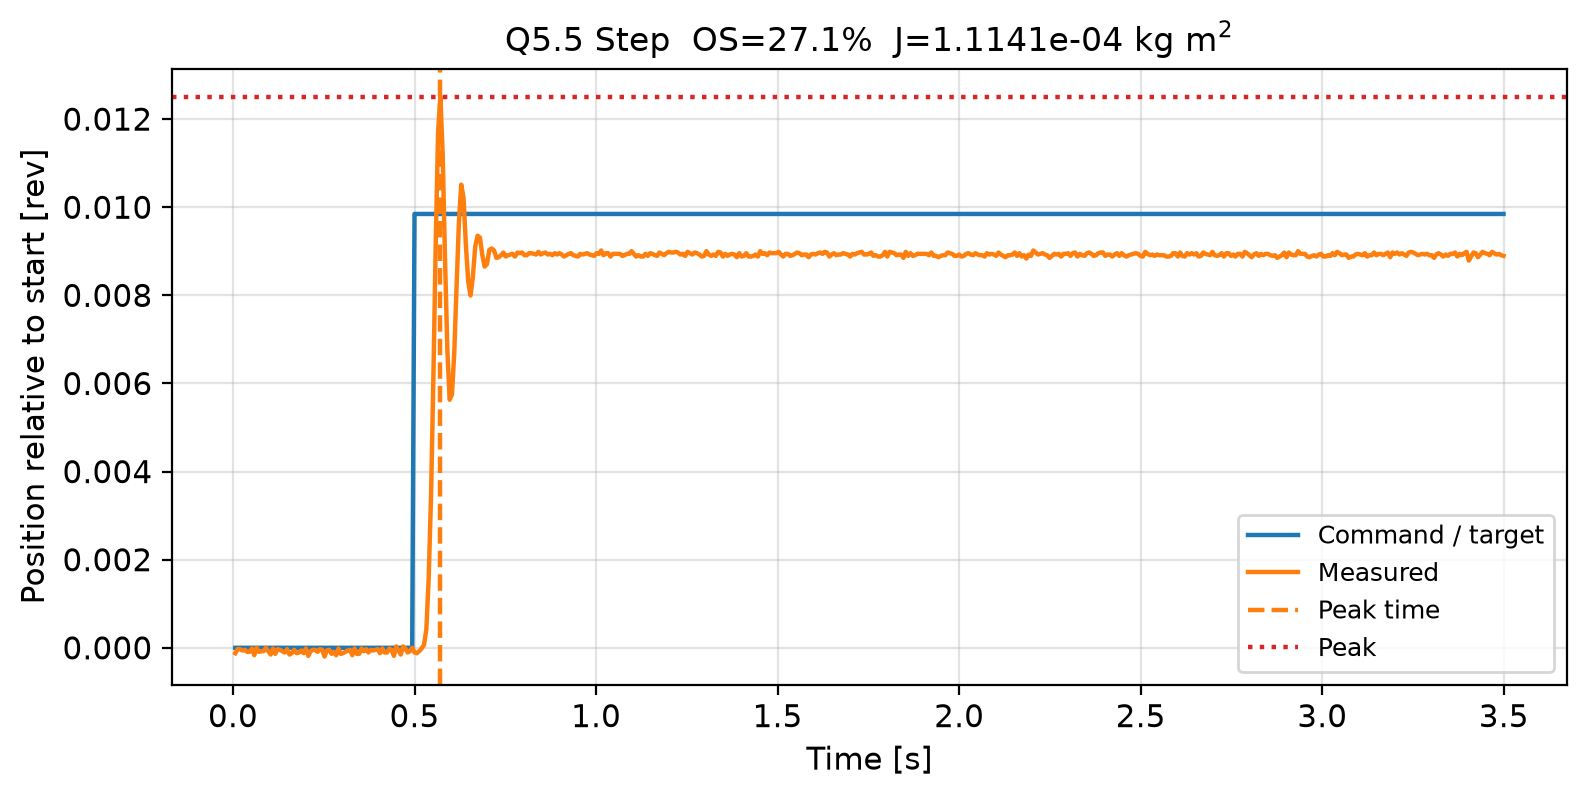
\includegraphics[width=0.85\textwidth]{Plots/section5_5_step.png}
  \caption{Step response used for the inertia estimate (visible overshoot).}
  \label{fig:q55}
\end{figure}

\begin{table}[H]
\centering
\caption{Rotor inertia from step response and from calipers.}
\begin{tabular}{lll}
\toprule
Method & $J$ (\si{\kilogram\meter\squared}) & Notes \\
\midrule
Step response & $1.11\times 10^{-4}$ & $M_p=27\%$, $t_p=71\,\mathrm{ms}$ \\
Thin steel ring & $5.92\times 10^{-5}$ & $\rho=7800$, OD/wall/axial $63/4/11.7\,\mathrm{mm}$ \\
\bottomrule
\end{tabular}
\end{table}

% ============================================================
\section{Frequency Response and Bandwidth}
% ============================================================

\question{Q6.1}{Plot magnitude in dB and phase in degrees against frequency on a
log axis. Report the \SI{-3}{\decibel} bandwidth and the peak magnitude.}

\solution

\begin{figure}[H]
  \centering
  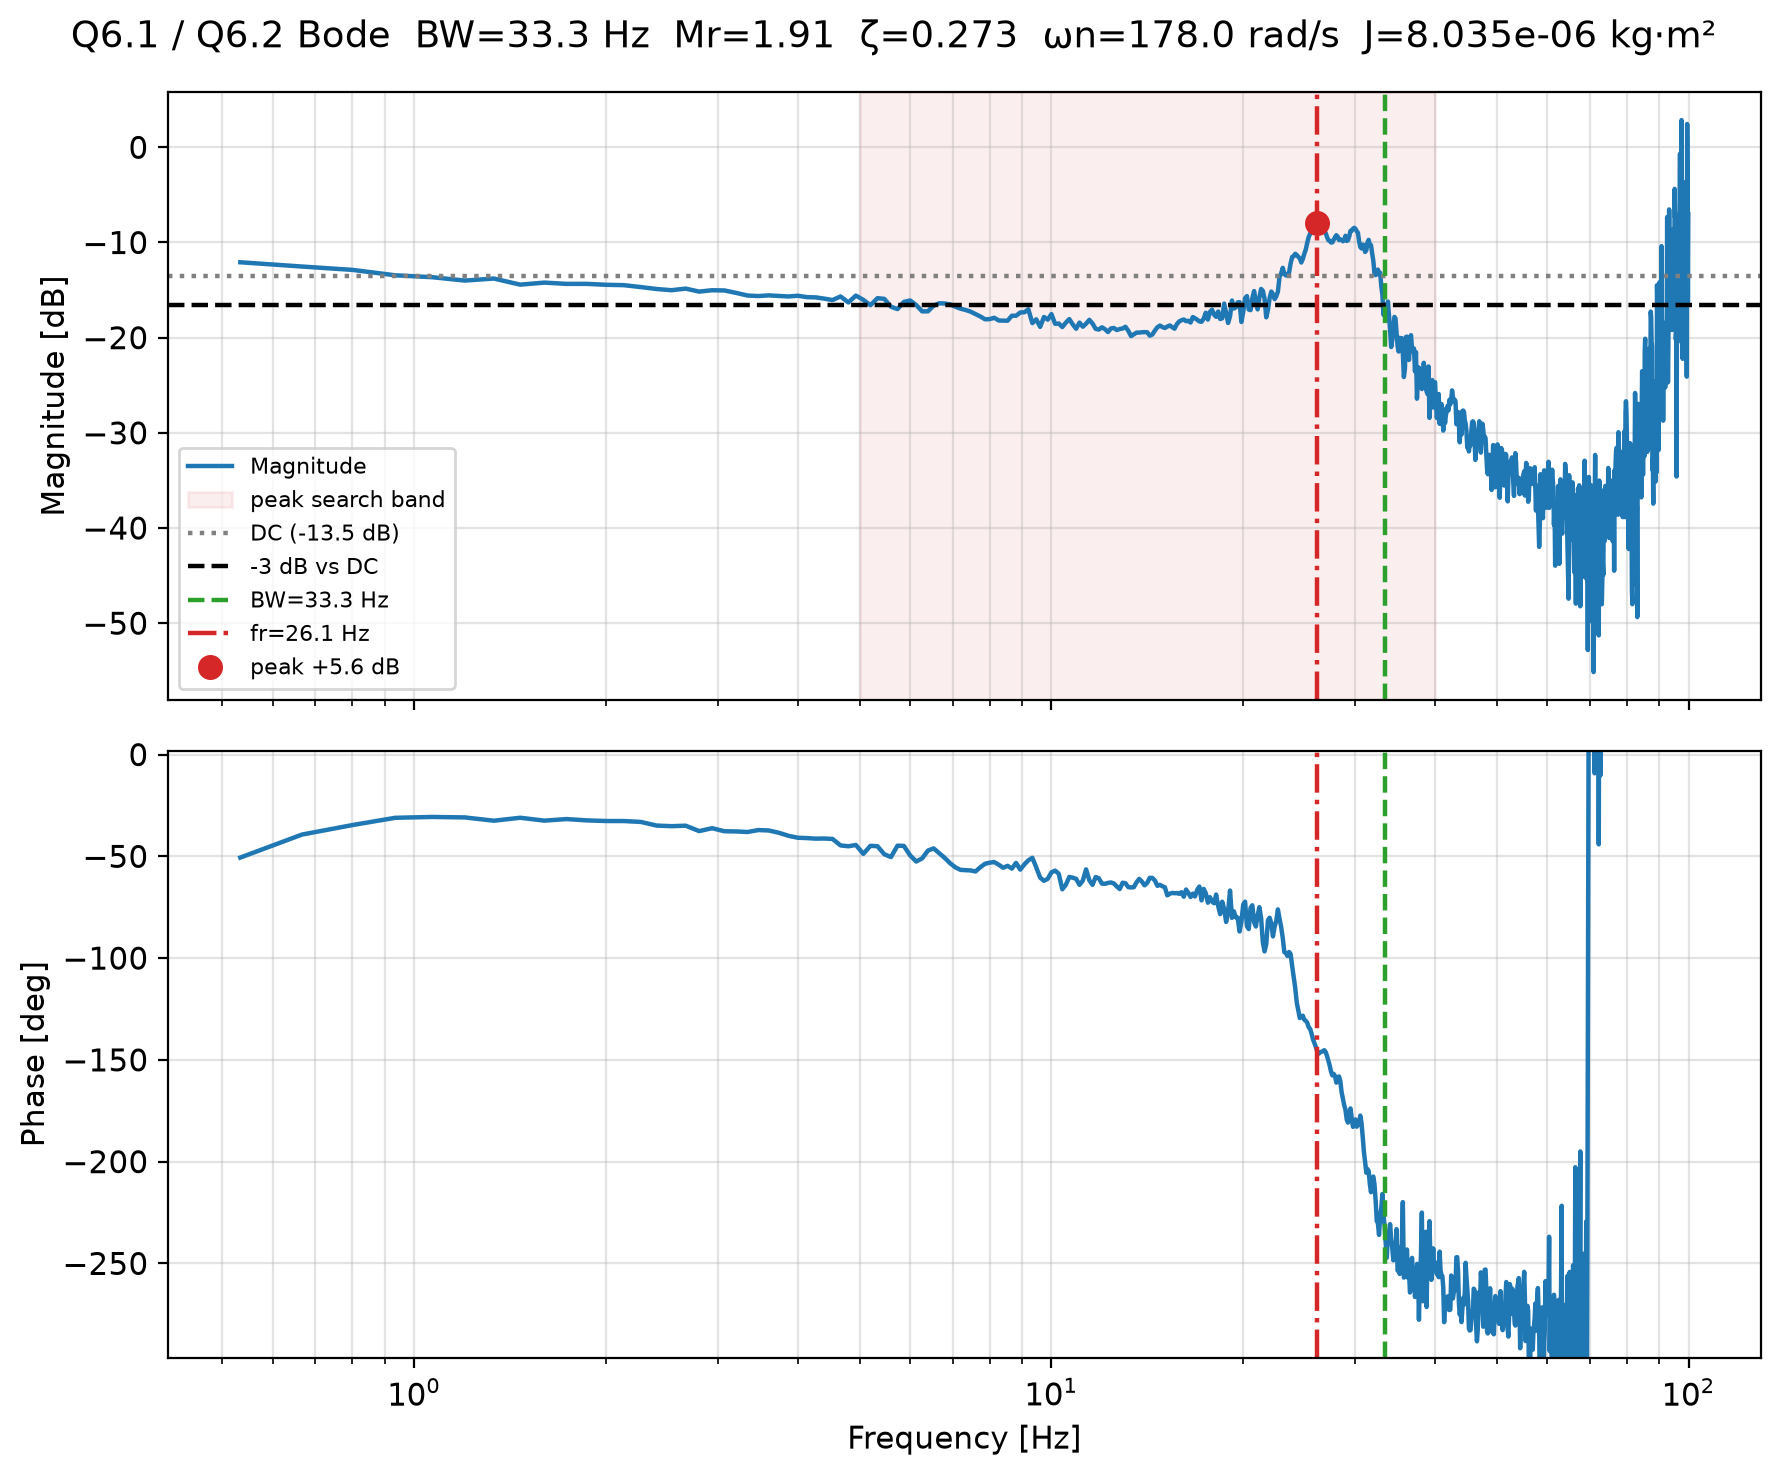
\includegraphics[width=0.9\textwidth]{Plots/section6_1_bode.png}
  \caption{Closed-loop frequency response from a chirp, \SI{0.5}{\hertz} to
  \SI{100}{\hertz}.}
  \label{fig:q61}
\end{figure}

\begin{table}[H]
\centering
\caption{Closed-loop bandwidth metrics.}
\begin{tabular}{ll}
\toprule
Quantity & Value \\
\midrule
\SI{-3}{\decibel} bandwidth & \SI{32.4}{\hertz} \\
Peak magnitude & \SI{-7.37}{\decibel} (\SI{+4.18}{\decibel} vs DC) \\
\bottomrule
\end{tabular}
\end{table}

% ANSWER. State the chirp amplitude and your sample rate, and do not plot above
% roughly f_s/5.

\question{Q6.2}{Extract the natural frequency and damping ratio from the
frequency response. Use them with your gains to compute the rotor inertia a
second time. Compare against Q5.5 and report the difference as a percentage.
Should the two agree? Why or why not?}

\solution

\begin{align*}
  M_r &= \frac{1}{2\zeta\sqrt{1-\zeta^2}}, &
  \omega_r &= \omega_n\sqrt{1-2\zeta^2}
\end{align*}

From the Bode peak: $M_r = 1.62$ ($+4.18\,\mathrm{dB}$), $f_r = 24.9\,\mathrm{Hz}$
$\Rightarrow$ $\zeta = 0.327$, $\omega_n = 177\,\mathrm{rad/s}$,
$J_{\text{chirp}} = 8.16\times 10^{-6}\,\mathrm{kg\,m^2}$
(about $93\%$ lower than the Q5.5 step value --- the two need not agree
exactly: CSD estimates, gain mismatch, and unmodelled dynamics all bias
$\omega_n$).

\begin{table}[H]
\centering
\caption{Inertia from frequency response versus step response.}
\begin{tabular}{lll}
\toprule
Source & $J$ (\si{\kilogram\meter\squared}) & Difference \\
\midrule
Q5.5 step & $1.11\times 10^{-4}$ & --- \\
Q6.2 chirp & $8.16\times 10^{-6}$ & $-92.7\%$ \\
\bottomrule
\end{tabular}
\end{table}

% ============================================================
\section{Identifying an Inertia}
% ============================================================

\paragraph{Disk mass and CAD value.}
Measured disk mass: \SI{72.4}{\gram}.
\begin{equation*}
  J_{\text{disk,CAD}} = 6.6185\times10^{-5} \times
    \frac{m_{\text{measured}}}{\SI{76.85}{\gram}}
    = 6.6185\times10^{-5} \times \frac{72.4}{76.85}
    = 6.24\times10^{-5}\,\mathrm{kg\,m^2}
\end{equation*}

\question{P7.1}{Predict what mounting the disk will do to the natural frequency,
the damping ratio, and the overshoot of your step response. No numbers. Give a
direction and a reason for each.}

\begin{prediction}
\begin{table}[H]
\centering
\begin{tabular}{lll}
\toprule
Quantity & Direction & Reason \\
\midrule
$\omega_n$ & & \\
$\zeta$    & & \\
Overshoot  & & \\
\bottomrule
\end{tabular}
\end{table}
\end{prediction}

\question{Q7.1}{Use the measured natural frequency and overshoot to compute the
inertia of the disk. Derive the relation you use. Compare against the value
given at the top of this section. Why would a value you got through the control
loop differ from one you got by measuring the object? What does that imply about
identifying a system through its own controller?}

\solution

\begin{equation*}
  \frac{\omega_{n,\text{bare}}}{\omega_{n,\text{loaded}}}
    = \sqrt{\frac{J_{\text{rotor}} + J_{\text{disk}}}{J_{\text{rotor}}}}
  \quad\Rightarrow\quad
  J_{\text{disk}} = J_{\text{rotor}}
    \left[\left(\frac{\omega_{n,\text{bare}}}{\omega_{n,\text{loaded}}}\right)^{\!2} - 1\right]
\end{equation*}

\begin{figure}[H]
  \centering
  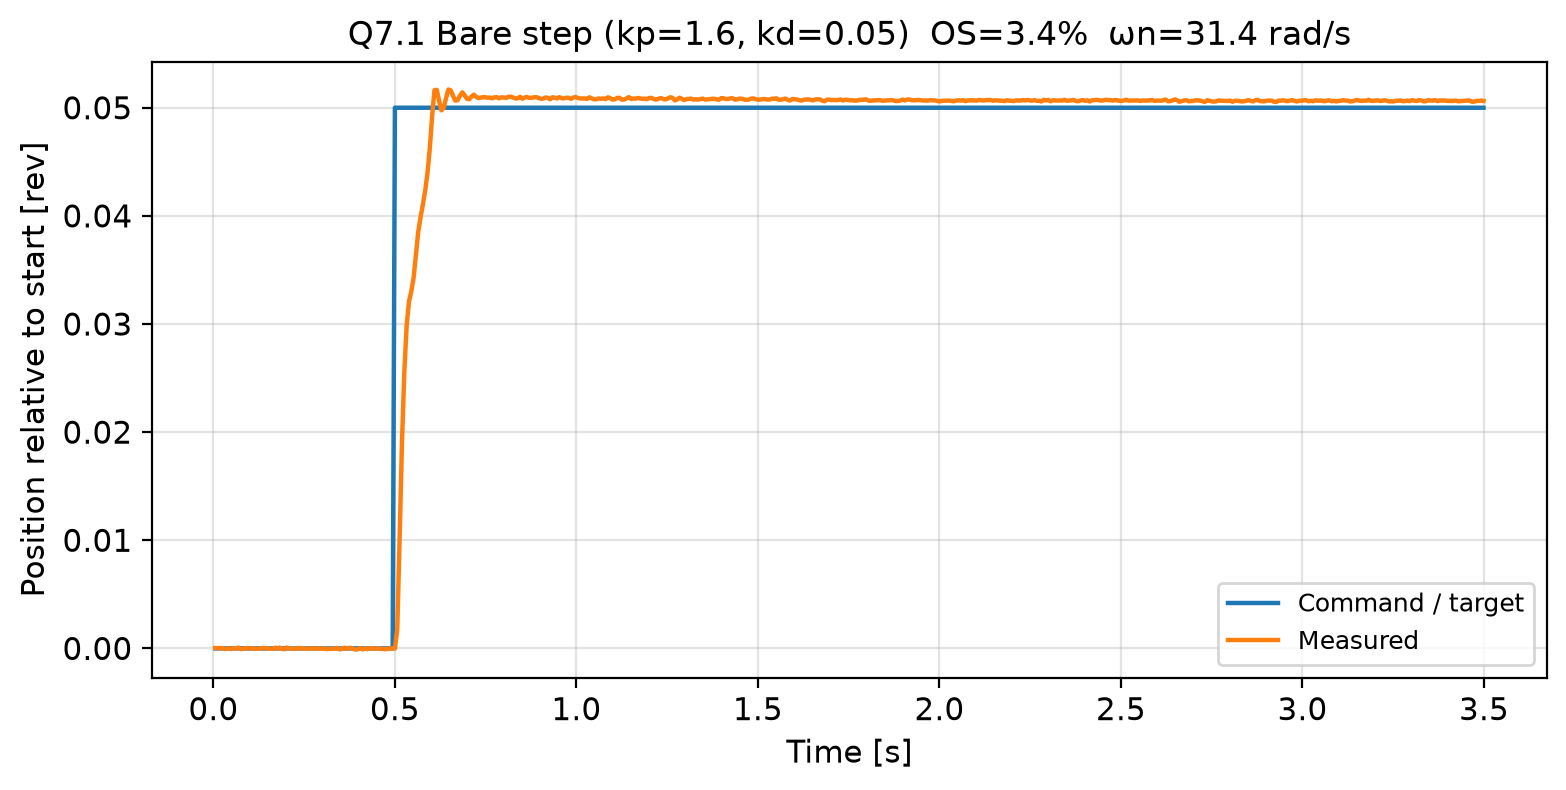
\includegraphics[width=0.85\textwidth]{Plots/section7_1_step_bare.png}
  \caption{Bare-shaft step response baseline before mounting the disk.}
  \label{fig:q71a}
\end{figure}

\begin{figure}[H]
  \centering
  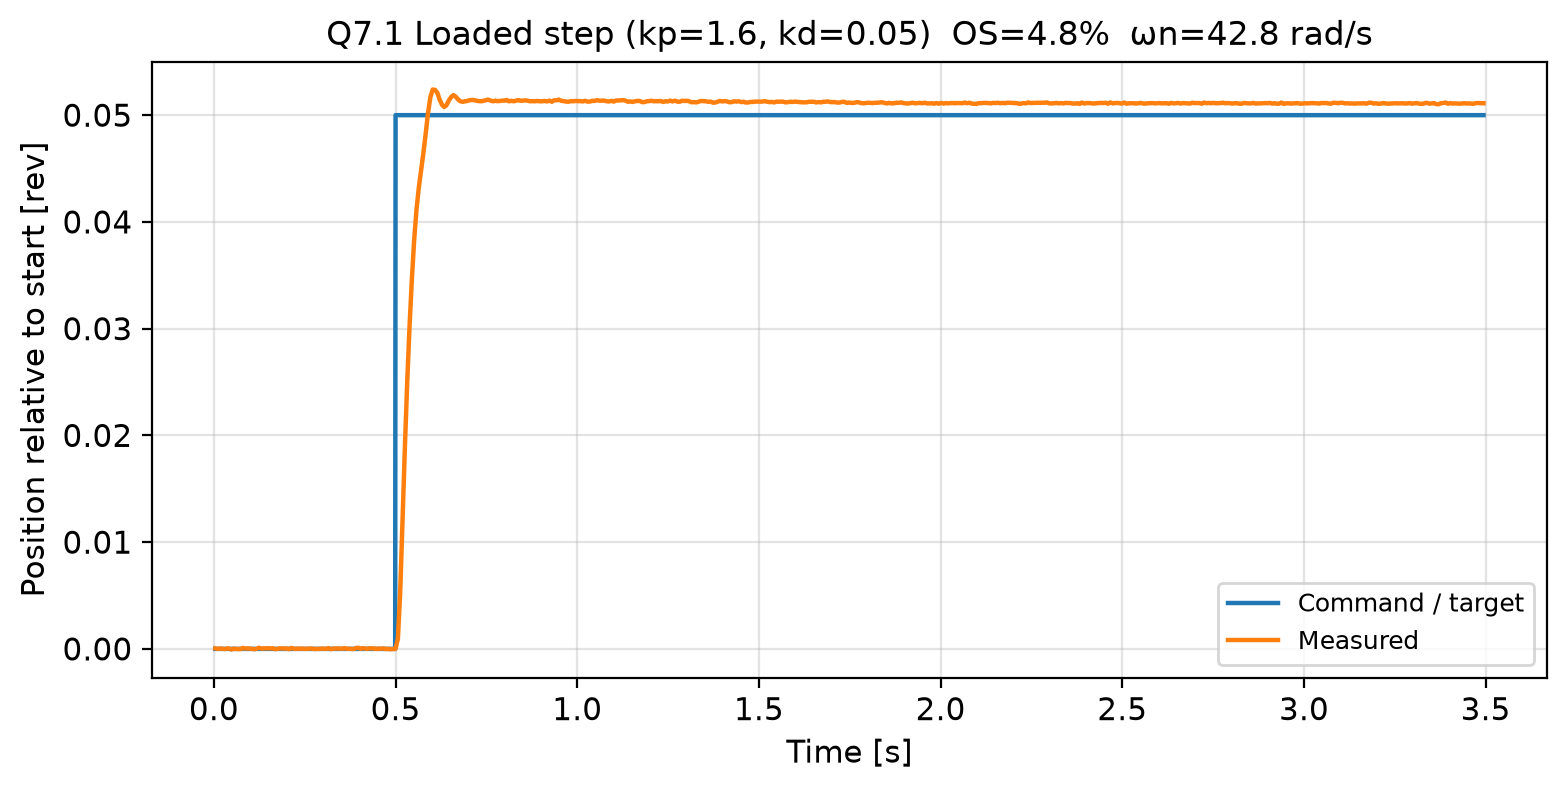
\includegraphics[width=0.85\textwidth]{Plots/section7_1_step_loaded.png}
  \caption{Step response with the inertia disk mounted (gains unchanged).}
  \label{fig:q71b}
\end{figure}

\begin{table}[H]
\centering
\caption{Disk inertia from the control loop versus CAD scaling.}
\begin{tabular}{lll}
\toprule
Method & $J_{\text{disk}}$ (\si{\kilogram\meter\squared}) & Notes \\
\midrule
Frequency / overshoot ratio & $1.21\times 10^{-5}$ & $\omega_{n,\text{bare}}/\omega_{n,\text{loaded}}$ \\
$J_{\text{total}} - J_{\text{rotor}}$ & $1.21\times 10^{-5}$ & same as above \\
CAD $\times$ measured mass & $6.24\times 10^{-5}$ & $m=72.4\,\mathrm{g}$ \\
\bottomrule
\end{tabular}
\end{table}

\question{Q7.2}{With the disk installed, retune $k_p$ and $k_d$ to get as close
to your original bandwidth and damping ratio as you can. Report the new gains.
How does adding inertia to the rotor affect motor performance?}

\solution

\begin{equation*}
  \alpha = \frac{J_{\text{rotor}} + J_{\text{disk}}}{J_{\text{rotor}}}
    = \left(\frac{\omega_{n,\text{bare}}}{\omega_{n,\text{loaded}}}\right)^{2}
    \approx 1.109,
  \qquad k_p' = \alpha k_p, \qquad k_d' = \alpha k_d
\end{equation*}

Adding inertia lowers $\omega_n$ at fixed gains, so the motor feels slower and
less responsive. Scaling $k_p$ and $k_d$ by $\alpha$ restores the closed-loop
natural frequency and damping (to first order).

\begin{table}[H]
\centering
\caption{Retuned gains with the disk installed.}
\begin{tabular}{lll}
\toprule
 & Predicted ($\times\alpha$) & Measured \\
\midrule
$k_p$ & $1.77$ &  \\
$k_d$ & $0.0554$ &  \\
$k_i$ & $2.97$ &  \\
\bottomrule
\end{tabular}
\end{table}

\begin{figure}[H]
  \centering
  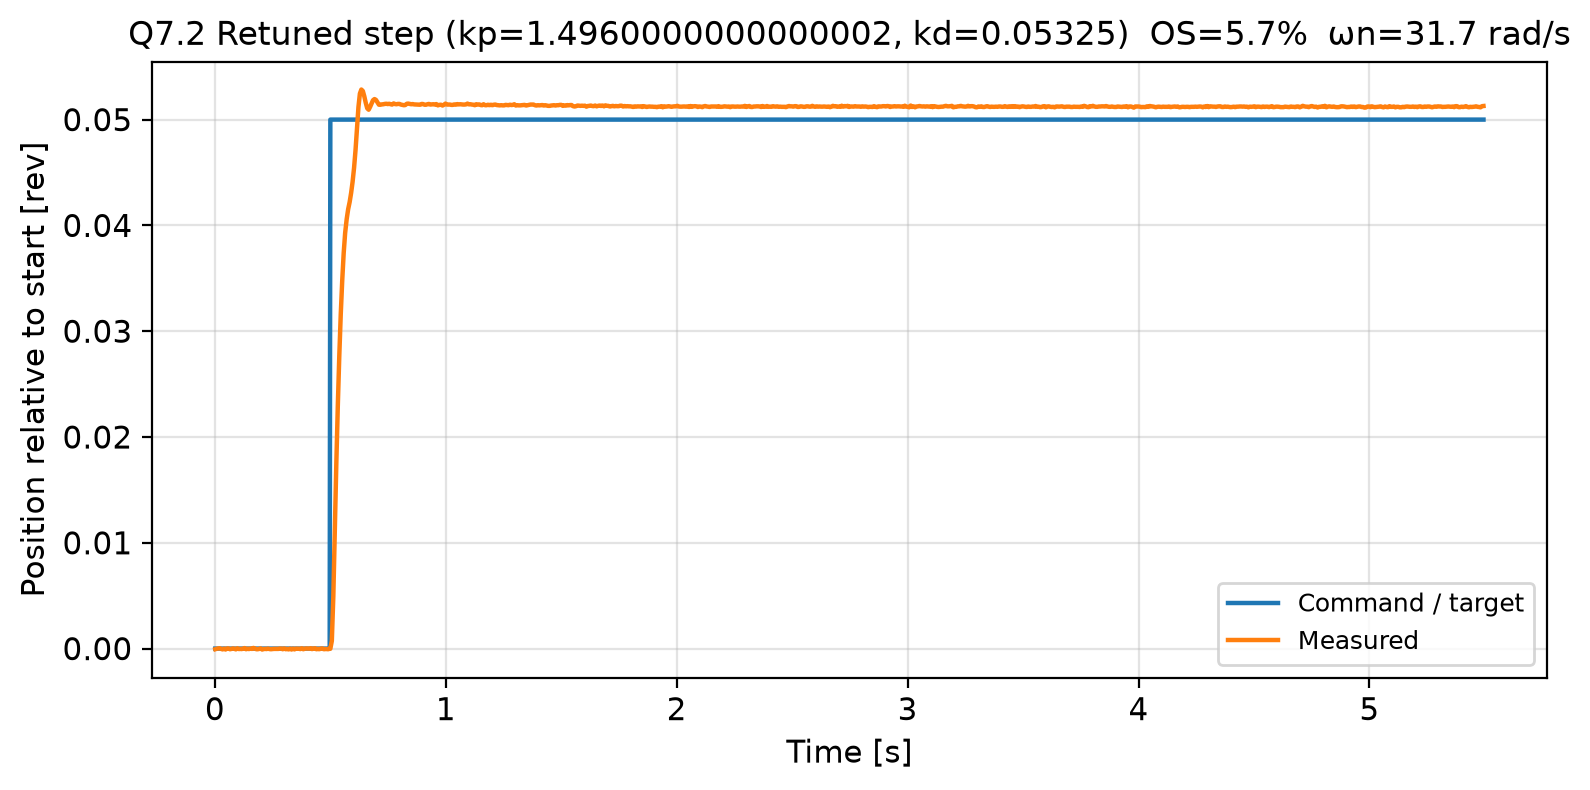
\includegraphics[width=0.85\textwidth]{Plots/section7_2_step_retuned.png}
  \caption{Step response after retuning $k_p$ and $k_d$ with the disk installed.}
  \label{fig:q72}
\end{figure}

% ============================================================
\section{Consistency Across Sections}
% ============================================================
% Not asked for. Worth including: it is what makes the report read as one
% investigation rather than seven exercises.

\begin{table}[H]
\centering
\caption{The same quantities measured by independent methods.}
\small
\begin{tabular}{lllll}
\toprule
Quantity & Method A & Method B & Method C & Explanation of the gap \\
\midrule
$K_t$            & datasheet & calibration & scale & \\
Pole pairs       & Q1.1 & Q3.2 & --- & \\
$J_{\text{rotor}}$ & Q5.5 step & Q6.2 chirp & calipers & \\
$J_{\text{disk}}$  & Q7.1 loop & CAD + mass & --- & \\
Friction torque  & Q2.2 hysteresis & Q5.2 park-short & --- & \\
Command rate     & Q4.4 calculated & Q1.3 achieved & capture timestamps & \\
\bottomrule
\end{tabular}
\end{table}

% Closing paragraph: identifying a plant through its own controller measures the
% plant convolved with everything the controller believes about it.

% ============================================================
\appendix
\section{Calibration Console Output}
% \lstinputlisting{data/calibration.txt}

\section{Scripts}
% Not required for submission. Include only if it helps the reader.

\end{document}